\documentclass[10pt]{article}
\usepackage[a4paper,margin=15mm]{geometry}
\usepackage{tikz}
\usetikzlibrary{decorations.pathmorphing,decorations.markings}
\tikzset{
  photon/.style={decorate,decoration={snake,amplitude=0.55mm,segment length=1.8mm,pre length=0.3mm,post length=0.3mm}},
  fermion/.style={thick,postaction={decorate},decoration={markings,mark=at position 0.55 with {\arrow{stealth}}}},
  eline/.style={thick},
  vtx/.style={circle,fill,inner sep=0.8pt},
  bubble/.style={circle,draw,thick,fill=white,minimum size=5.6mm,inner sep=0pt},
}
\newcommand{\dcell}[2]{\begin{minipage}[t]{0.24\textwidth}\centering #1\\[0.5mm]{\scriptsize #2}\end{minipage}}
\setlength{\parindent}{0pt}
\begin{document}
\section*{Diagrams evaluated by \texttt{sincqed}}
Each diagram is labelled by the program entry that evaluates it, its Volkov string
(external-photon vertex; photon ends, counting vertices along the electron line from 1) and,
in brackets, the weight with which that entry already includes it.  Entries of weight 2
include the mirror diagram, drawn next to its representative.  Electron loops are drawn as
circles (one-loop vacuum polarization), a circle with an internal photon (two-loop vacuum
polarization), or a box (light-by-light).

\subsection*{Two loops (7 diagrams)}
\dcell{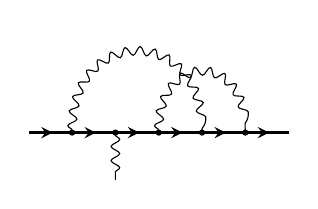
\begin{tikzpicture}[scale=0.55,baseline=(current bounding box.south)]
\draw[fermion] (0,0) -- (1,0);
\draw[fermion] (1,0) -- (2,0);
\draw[fermion] (2,0) -- (3,0);
\draw[fermion] (3,0) -- (4,0);
\draw[fermion] (4,0) -- (5,0);
\draw[fermion] (5,0) -- (6,0);
\draw[photon] (2,0) -- (2,-1.1);
\draw[photon] (1,0) .. controls (1,2.41) and (4,2.41) .. (4,0);
\draw[photon] (3,0) .. controls (3,1.79) and (5,1.79) .. (5,0);
\node[vtx] at (1,0) {};
\node[vtx] at (2,0) {};
\node[vtx] at (3,0) {};
\node[vtx] at (4,0) {};
\node[vtx] at (5,0) {};
\end{tikzpicture}}{\texttt{g2\_00}\ \ 2; 1-4, 3-5\ \ [2]}\hfill\dcell{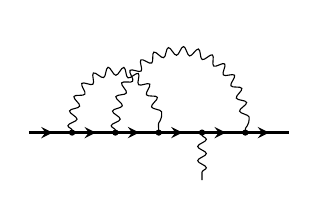
\begin{tikzpicture}[scale=0.55,baseline=(current bounding box.south)]
\draw[fermion] (0,0) -- (1,0);
\draw[fermion] (1,0) -- (2,0);
\draw[fermion] (2,0) -- (3,0);
\draw[fermion] (3,0) -- (4,0);
\draw[fermion] (4,0) -- (5,0);
\draw[fermion] (5,0) -- (6,0);
\draw[photon] (4,0) -- (4,-1.1);
\draw[photon] (1,0) .. controls (1,1.79) and (3,1.79) .. (3,0);
\draw[photon] (2,0) .. controls (2,2.41) and (5,2.41) .. (5,0);
\node[vtx] at (1,0) {};
\node[vtx] at (2,0) {};
\node[vtx] at (3,0) {};
\node[vtx] at (4,0) {};
\node[vtx] at (5,0) {};
\end{tikzpicture}}{\texttt{g2\_00} mirror: 4; 1-3, 2-5}\hfill\dcell{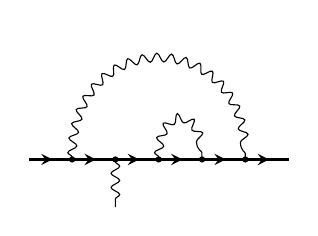
\begin{tikzpicture}[scale=0.55,baseline=(current bounding box.south)]
\draw[fermion] (0,0) -- (1,0);
\draw[fermion] (1,0) -- (2,0);
\draw[fermion] (2,0) -- (3,0);
\draw[fermion] (3,0) -- (4,0);
\draw[fermion] (4,0) -- (5,0);
\draw[fermion] (5,0) -- (6,0);
\draw[photon] (2,0) -- (2,-1.1);
\draw[photon] (1,0) .. controls (1,3.03) and (5,3.03) .. (5,0);
\draw[photon] (3,0) .. controls (3,1.17) and (4,1.17) .. (4,0);
\node[vtx] at (1,0) {};
\node[vtx] at (2,0) {};
\node[vtx] at (3,0) {};
\node[vtx] at (4,0) {};
\node[vtx] at (5,0) {};
\end{tikzpicture}}{\texttt{g2\_01}\ \ 2; 1-5, 3-4\ \ [2]}\hfill\dcell{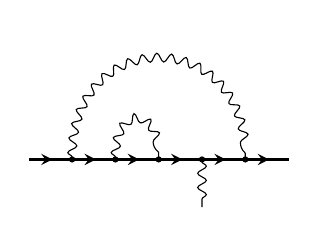
\begin{tikzpicture}[scale=0.55,baseline=(current bounding box.south)]
\draw[fermion] (0,0) -- (1,0);
\draw[fermion] (1,0) -- (2,0);
\draw[fermion] (2,0) -- (3,0);
\draw[fermion] (3,0) -- (4,0);
\draw[fermion] (4,0) -- (5,0);
\draw[fermion] (5,0) -- (6,0);
\draw[photon] (4,0) -- (4,-1.1);
\draw[photon] (1,0) .. controls (1,3.03) and (5,3.03) .. (5,0);
\draw[photon] (2,0) .. controls (2,1.17) and (3,1.17) .. (3,0);
\node[vtx] at (1,0) {};
\node[vtx] at (2,0) {};
\node[vtx] at (3,0) {};
\node[vtx] at (4,0) {};
\node[vtx] at (5,0) {};
\end{tikzpicture}}{\texttt{g2\_01} mirror: 4; 1-5, 2-3}\hfill\mbox{}\par\vspace{3mm}
\dcell{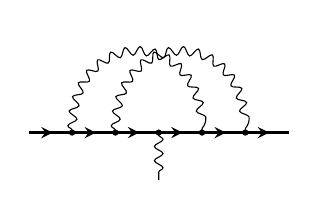
\begin{tikzpicture}[scale=0.55,baseline=(current bounding box.south)]
\draw[fermion] (0,0) -- (1,0);
\draw[fermion] (1,0) -- (2,0);
\draw[fermion] (2,0) -- (3,0);
\draw[fermion] (3,0) -- (4,0);
\draw[fermion] (4,0) -- (5,0);
\draw[fermion] (5,0) -- (6,0);
\draw[photon] (3,0) -- (3,-1.1);
\draw[photon] (1,0) .. controls (1,2.41) and (4,2.41) .. (4,0);
\draw[photon] (2,0) .. controls (2,2.41) and (5,2.41) .. (5,0);
\node[vtx] at (1,0) {};
\node[vtx] at (2,0) {};
\node[vtx] at (3,0) {};
\node[vtx] at (4,0) {};
\node[vtx] at (5,0) {};
\end{tikzpicture}}{\texttt{g2\_02}\ \ 3; 1-4, 2-5\ \ [1]}\hfill\dcell{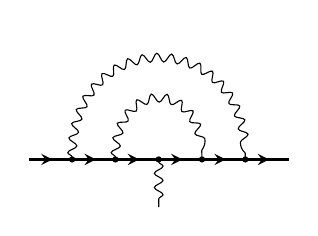
\begin{tikzpicture}[scale=0.55,baseline=(current bounding box.south)]
\draw[fermion] (0,0) -- (1,0);
\draw[fermion] (1,0) -- (2,0);
\draw[fermion] (2,0) -- (3,0);
\draw[fermion] (3,0) -- (4,0);
\draw[fermion] (4,0) -- (5,0);
\draw[fermion] (5,0) -- (6,0);
\draw[photon] (3,0) -- (3,-1.1);
\draw[photon] (1,0) .. controls (1,3.03) and (5,3.03) .. (5,0);
\draw[photon] (2,0) .. controls (2,1.79) and (4,1.79) .. (4,0);
\node[vtx] at (1,0) {};
\node[vtx] at (2,0) {};
\node[vtx] at (3,0) {};
\node[vtx] at (4,0) {};
\node[vtx] at (5,0) {};
\end{tikzpicture}}{\texttt{g2\_03}\ \ 3; 1-5, 2-4\ \ [1]}\hfill\dcell{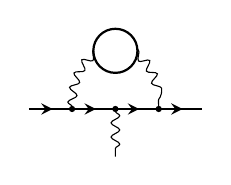
\begin{tikzpicture}[scale=0.55,baseline=(current bounding box.south)]
\draw[fermion] (0,0) -- (1,0);
\draw[fermion] (1,0) -- (2,0);
\draw[fermion] (2,0) -- (3,0);
\draw[fermion] (3,0) -- (4,0);
\draw[photon] (2,0) -- (2,-1.1);
\draw[photon] (1,0) .. controls (1,1.79) and (3,1.79) .. (3,0);
\node[bubble] (B005) at (2.000,1.343) {};
\node[vtx] at (1,0) {};
\node[vtx] at (2,0) {};
\node[vtx] at (3,0) {};
\end{tikzpicture}}{\texttt{v2\_00}\ \ one-loop VP [1]}\hfill\mbox{}\par\vspace{3mm}
\subsection*{Three loops without lepton loops (50 diagrams, group \texttt{q3})}
\dcell{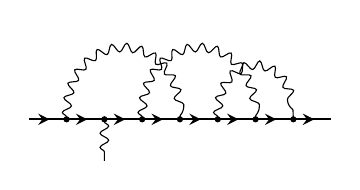
\begin{tikzpicture}[scale=0.48,baseline=(current bounding box.south)]
\draw[fermion] (0,0) -- (1,0);
\draw[fermion] (1,0) -- (2,0);
\draw[fermion] (2,0) -- (3,0);
\draw[fermion] (3,0) -- (4,0);
\draw[fermion] (4,0) -- (5,0);
\draw[fermion] (5,0) -- (6,0);
\draw[fermion] (6,0) -- (7,0);
\draw[fermion] (7,0) -- (8,0);
\draw[photon] (2,0) -- (2,-1.1);
\draw[photon] (1,0) .. controls (1,2.41) and (4,2.41) .. (4,0);
\draw[photon] (3,0) .. controls (3,2.41) and (6,2.41) .. (6,0);
\draw[photon] (5,0) .. controls (5,1.79) and (7,1.79) .. (7,0);
\node[vtx] at (1,0) {};
\node[vtx] at (2,0) {};
\node[vtx] at (3,0) {};
\node[vtx] at (4,0) {};
\node[vtx] at (5,0) {};
\node[vtx] at (6,0) {};
\node[vtx] at (7,0) {};
\end{tikzpicture}}{\texttt{g3\_00}\ \ 2; 1-4, 3-6, 5-7\ \ [2]}\hfill\dcell{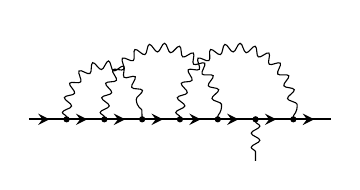
\begin{tikzpicture}[scale=0.48,baseline=(current bounding box.south)]
\draw[fermion] (0,0) -- (1,0);
\draw[fermion] (1,0) -- (2,0);
\draw[fermion] (2,0) -- (3,0);
\draw[fermion] (3,0) -- (4,0);
\draw[fermion] (4,0) -- (5,0);
\draw[fermion] (5,0) -- (6,0);
\draw[fermion] (6,0) -- (7,0);
\draw[fermion] (7,0) -- (8,0);
\draw[photon] (6,0) -- (6,-1.1);
\draw[photon] (1,0) .. controls (1,1.79) and (3,1.79) .. (3,0);
\draw[photon] (2,0) .. controls (2,2.41) and (5,2.41) .. (5,0);
\draw[photon] (4,0) .. controls (4,2.41) and (7,2.41) .. (7,0);
\node[vtx] at (1,0) {};
\node[vtx] at (2,0) {};
\node[vtx] at (3,0) {};
\node[vtx] at (4,0) {};
\node[vtx] at (5,0) {};
\node[vtx] at (6,0) {};
\node[vtx] at (7,0) {};
\end{tikzpicture}}{\texttt{g3\_00} mirror: 6; 1-3, 2-5, 4-7}\hfill\dcell{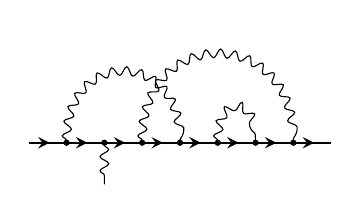
\begin{tikzpicture}[scale=0.48,baseline=(current bounding box.south)]
\draw[fermion] (0,0) -- (1,0);
\draw[fermion] (1,0) -- (2,0);
\draw[fermion] (2,0) -- (3,0);
\draw[fermion] (3,0) -- (4,0);
\draw[fermion] (4,0) -- (5,0);
\draw[fermion] (5,0) -- (6,0);
\draw[fermion] (6,0) -- (7,0);
\draw[fermion] (7,0) -- (8,0);
\draw[photon] (2,0) -- (2,-1.1);
\draw[photon] (1,0) .. controls (1,2.41) and (4,2.41) .. (4,0);
\draw[photon] (3,0) .. controls (3,3.03) and (7,3.03) .. (7,0);
\draw[photon] (5,0) .. controls (5,1.17) and (6,1.17) .. (6,0);
\node[vtx] at (1,0) {};
\node[vtx] at (2,0) {};
\node[vtx] at (3,0) {};
\node[vtx] at (4,0) {};
\node[vtx] at (5,0) {};
\node[vtx] at (6,0) {};
\node[vtx] at (7,0) {};
\end{tikzpicture}}{\texttt{g3\_01}\ \ 2; 1-4, 3-7, 5-6\ \ [2]}\hfill\dcell{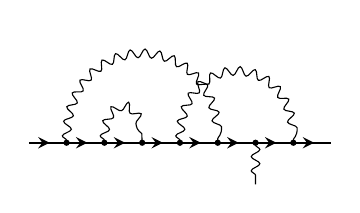
\begin{tikzpicture}[scale=0.48,baseline=(current bounding box.south)]
\draw[fermion] (0,0) -- (1,0);
\draw[fermion] (1,0) -- (2,0);
\draw[fermion] (2,0) -- (3,0);
\draw[fermion] (3,0) -- (4,0);
\draw[fermion] (4,0) -- (5,0);
\draw[fermion] (5,0) -- (6,0);
\draw[fermion] (6,0) -- (7,0);
\draw[fermion] (7,0) -- (8,0);
\draw[photon] (6,0) -- (6,-1.1);
\draw[photon] (1,0) .. controls (1,3.03) and (5,3.03) .. (5,0);
\draw[photon] (2,0) .. controls (2,1.17) and (3,1.17) .. (3,0);
\draw[photon] (4,0) .. controls (4,2.41) and (7,2.41) .. (7,0);
\node[vtx] at (1,0) {};
\node[vtx] at (2,0) {};
\node[vtx] at (3,0) {};
\node[vtx] at (4,0) {};
\node[vtx] at (5,0) {};
\node[vtx] at (6,0) {};
\node[vtx] at (7,0) {};
\end{tikzpicture}}{\texttt{g3\_01} mirror: 6; 1-5, 2-3, 4-7}\hfill\mbox{}\par\vspace{3mm}
\dcell{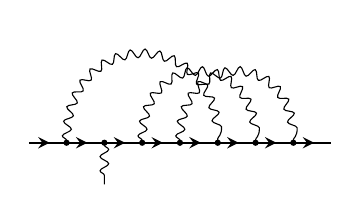
\begin{tikzpicture}[scale=0.48,baseline=(current bounding box.south)]
\draw[fermion] (0,0) -- (1,0);
\draw[fermion] (1,0) -- (2,0);
\draw[fermion] (2,0) -- (3,0);
\draw[fermion] (3,0) -- (4,0);
\draw[fermion] (4,0) -- (5,0);
\draw[fermion] (5,0) -- (6,0);
\draw[fermion] (6,0) -- (7,0);
\draw[fermion] (7,0) -- (8,0);
\draw[photon] (2,0) -- (2,-1.1);
\draw[photon] (1,0) .. controls (1,3.03) and (5,3.03) .. (5,0);
\draw[photon] (3,0) .. controls (3,2.41) and (6,2.41) .. (6,0);
\draw[photon] (4,0) .. controls (4,2.41) and (7,2.41) .. (7,0);
\node[vtx] at (1,0) {};
\node[vtx] at (2,0) {};
\node[vtx] at (3,0) {};
\node[vtx] at (4,0) {};
\node[vtx] at (5,0) {};
\node[vtx] at (6,0) {};
\node[vtx] at (7,0) {};
\end{tikzpicture}}{\texttt{g3\_02}\ \ 2; 1-5, 3-6, 4-7\ \ [2]}\hfill\dcell{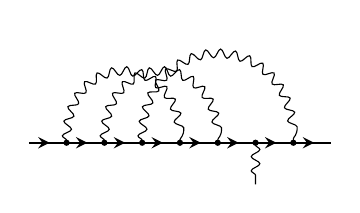
\begin{tikzpicture}[scale=0.48,baseline=(current bounding box.south)]
\draw[fermion] (0,0) -- (1,0);
\draw[fermion] (1,0) -- (2,0);
\draw[fermion] (2,0) -- (3,0);
\draw[fermion] (3,0) -- (4,0);
\draw[fermion] (4,0) -- (5,0);
\draw[fermion] (5,0) -- (6,0);
\draw[fermion] (6,0) -- (7,0);
\draw[fermion] (7,0) -- (8,0);
\draw[photon] (6,0) -- (6,-1.1);
\draw[photon] (1,0) .. controls (1,2.41) and (4,2.41) .. (4,0);
\draw[photon] (2,0) .. controls (2,2.41) and (5,2.41) .. (5,0);
\draw[photon] (3,0) .. controls (3,3.03) and (7,3.03) .. (7,0);
\node[vtx] at (1,0) {};
\node[vtx] at (2,0) {};
\node[vtx] at (3,0) {};
\node[vtx] at (4,0) {};
\node[vtx] at (5,0) {};
\node[vtx] at (6,0) {};
\node[vtx] at (7,0) {};
\end{tikzpicture}}{\texttt{g3\_02} mirror: 6; 1-4, 2-5, 3-7}\hfill\dcell{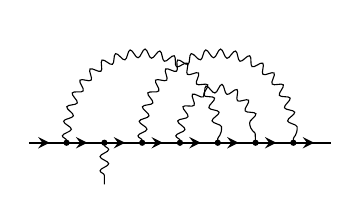
\begin{tikzpicture}[scale=0.48,baseline=(current bounding box.south)]
\draw[fermion] (0,0) -- (1,0);
\draw[fermion] (1,0) -- (2,0);
\draw[fermion] (2,0) -- (3,0);
\draw[fermion] (3,0) -- (4,0);
\draw[fermion] (4,0) -- (5,0);
\draw[fermion] (5,0) -- (6,0);
\draw[fermion] (6,0) -- (7,0);
\draw[fermion] (7,0) -- (8,0);
\draw[photon] (2,0) -- (2,-1.1);
\draw[photon] (1,0) .. controls (1,3.03) and (5,3.03) .. (5,0);
\draw[photon] (3,0) .. controls (3,3.03) and (7,3.03) .. (7,0);
\draw[photon] (4,0) .. controls (4,1.79) and (6,1.79) .. (6,0);
\node[vtx] at (1,0) {};
\node[vtx] at (2,0) {};
\node[vtx] at (3,0) {};
\node[vtx] at (4,0) {};
\node[vtx] at (5,0) {};
\node[vtx] at (6,0) {};
\node[vtx] at (7,0) {};
\end{tikzpicture}}{\texttt{g3\_03}\ \ 2; 1-5, 3-7, 4-6\ \ [2]}\hfill\dcell{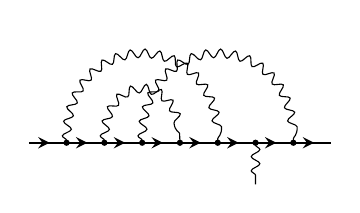
\begin{tikzpicture}[scale=0.48,baseline=(current bounding box.south)]
\draw[fermion] (0,0) -- (1,0);
\draw[fermion] (1,0) -- (2,0);
\draw[fermion] (2,0) -- (3,0);
\draw[fermion] (3,0) -- (4,0);
\draw[fermion] (4,0) -- (5,0);
\draw[fermion] (5,0) -- (6,0);
\draw[fermion] (6,0) -- (7,0);
\draw[fermion] (7,0) -- (8,0);
\draw[photon] (6,0) -- (6,-1.1);
\draw[photon] (1,0) .. controls (1,3.03) and (5,3.03) .. (5,0);
\draw[photon] (2,0) .. controls (2,1.79) and (4,1.79) .. (4,0);
\draw[photon] (3,0) .. controls (3,3.03) and (7,3.03) .. (7,0);
\node[vtx] at (1,0) {};
\node[vtx] at (2,0) {};
\node[vtx] at (3,0) {};
\node[vtx] at (4,0) {};
\node[vtx] at (5,0) {};
\node[vtx] at (6,0) {};
\node[vtx] at (7,0) {};
\end{tikzpicture}}{\texttt{g3\_03} mirror: 6; 1-5, 2-4, 3-7}\hfill\mbox{}\par\vspace{3mm}
\dcell{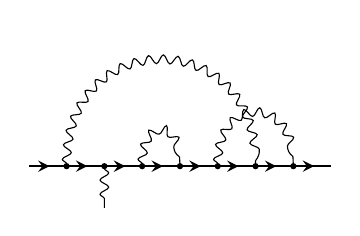
\begin{tikzpicture}[scale=0.48,baseline=(current bounding box.south)]
\draw[fermion] (0,0) -- (1,0);
\draw[fermion] (1,0) -- (2,0);
\draw[fermion] (2,0) -- (3,0);
\draw[fermion] (3,0) -- (4,0);
\draw[fermion] (4,0) -- (5,0);
\draw[fermion] (5,0) -- (6,0);
\draw[fermion] (6,0) -- (7,0);
\draw[fermion] (7,0) -- (8,0);
\draw[photon] (2,0) -- (2,-1.1);
\draw[photon] (1,0) .. controls (1,3.65) and (6,3.65) .. (6,0);
\draw[photon] (3,0) .. controls (3,1.17) and (4,1.17) .. (4,0);
\draw[photon] (5,0) .. controls (5,1.79) and (7,1.79) .. (7,0);
\node[vtx] at (1,0) {};
\node[vtx] at (2,0) {};
\node[vtx] at (3,0) {};
\node[vtx] at (4,0) {};
\node[vtx] at (5,0) {};
\node[vtx] at (6,0) {};
\node[vtx] at (7,0) {};
\end{tikzpicture}}{\texttt{g3\_04}\ \ 2; 1-6, 3-4, 5-7\ \ [2]}\hfill\dcell{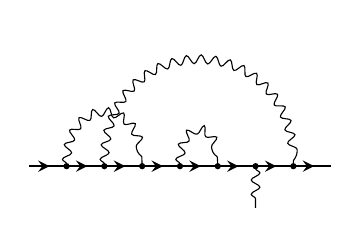
\begin{tikzpicture}[scale=0.48,baseline=(current bounding box.south)]
\draw[fermion] (0,0) -- (1,0);
\draw[fermion] (1,0) -- (2,0);
\draw[fermion] (2,0) -- (3,0);
\draw[fermion] (3,0) -- (4,0);
\draw[fermion] (4,0) -- (5,0);
\draw[fermion] (5,0) -- (6,0);
\draw[fermion] (6,0) -- (7,0);
\draw[fermion] (7,0) -- (8,0);
\draw[photon] (6,0) -- (6,-1.1);
\draw[photon] (1,0) .. controls (1,1.79) and (3,1.79) .. (3,0);
\draw[photon] (2,0) .. controls (2,3.65) and (7,3.65) .. (7,0);
\draw[photon] (4,0) .. controls (4,1.17) and (5,1.17) .. (5,0);
\node[vtx] at (1,0) {};
\node[vtx] at (2,0) {};
\node[vtx] at (3,0) {};
\node[vtx] at (4,0) {};
\node[vtx] at (5,0) {};
\node[vtx] at (6,0) {};
\node[vtx] at (7,0) {};
\end{tikzpicture}}{\texttt{g3\_04} mirror: 6; 1-3, 2-7, 4-5}\hfill\dcell{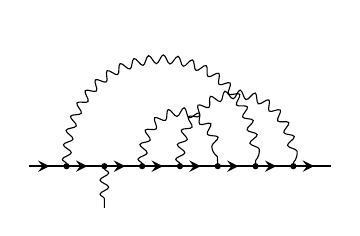
\begin{tikzpicture}[scale=0.48,baseline=(current bounding box.south)]
\draw[fermion] (0,0) -- (1,0);
\draw[fermion] (1,0) -- (2,0);
\draw[fermion] (2,0) -- (3,0);
\draw[fermion] (3,0) -- (4,0);
\draw[fermion] (4,0) -- (5,0);
\draw[fermion] (5,0) -- (6,0);
\draw[fermion] (6,0) -- (7,0);
\draw[fermion] (7,0) -- (8,0);
\draw[photon] (2,0) -- (2,-1.1);
\draw[photon] (1,0) .. controls (1,3.65) and (6,3.65) .. (6,0);
\draw[photon] (3,0) .. controls (3,1.79) and (5,1.79) .. (5,0);
\draw[photon] (4,0) .. controls (4,2.41) and (7,2.41) .. (7,0);
\node[vtx] at (1,0) {};
\node[vtx] at (2,0) {};
\node[vtx] at (3,0) {};
\node[vtx] at (4,0) {};
\node[vtx] at (5,0) {};
\node[vtx] at (6,0) {};
\node[vtx] at (7,0) {};
\end{tikzpicture}}{\texttt{g3\_05}\ \ 2; 1-6, 3-5, 4-7\ \ [2]}\hfill\dcell{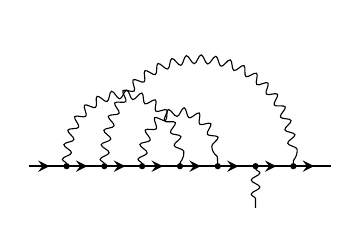
\begin{tikzpicture}[scale=0.48,baseline=(current bounding box.south)]
\draw[fermion] (0,0) -- (1,0);
\draw[fermion] (1,0) -- (2,0);
\draw[fermion] (2,0) -- (3,0);
\draw[fermion] (3,0) -- (4,0);
\draw[fermion] (4,0) -- (5,0);
\draw[fermion] (5,0) -- (6,0);
\draw[fermion] (6,0) -- (7,0);
\draw[fermion] (7,0) -- (8,0);
\draw[photon] (6,0) -- (6,-1.1);
\draw[photon] (1,0) .. controls (1,2.41) and (4,2.41) .. (4,0);
\draw[photon] (2,0) .. controls (2,3.65) and (7,3.65) .. (7,0);
\draw[photon] (3,0) .. controls (3,1.79) and (5,1.79) .. (5,0);
\node[vtx] at (1,0) {};
\node[vtx] at (2,0) {};
\node[vtx] at (3,0) {};
\node[vtx] at (4,0) {};
\node[vtx] at (5,0) {};
\node[vtx] at (6,0) {};
\node[vtx] at (7,0) {};
\end{tikzpicture}}{\texttt{g3\_05} mirror: 6; 1-4, 2-7, 3-5}\hfill\mbox{}\par\vspace{3mm}
\dcell{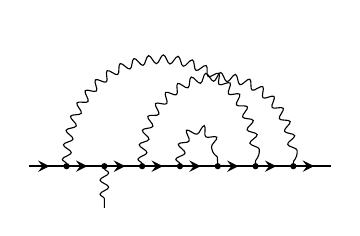
\begin{tikzpicture}[scale=0.48,baseline=(current bounding box.south)]
\draw[fermion] (0,0) -- (1,0);
\draw[fermion] (1,0) -- (2,0);
\draw[fermion] (2,0) -- (3,0);
\draw[fermion] (3,0) -- (4,0);
\draw[fermion] (4,0) -- (5,0);
\draw[fermion] (5,0) -- (6,0);
\draw[fermion] (6,0) -- (7,0);
\draw[fermion] (7,0) -- (8,0);
\draw[photon] (2,0) -- (2,-1.1);
\draw[photon] (1,0) .. controls (1,3.65) and (6,3.65) .. (6,0);
\draw[photon] (3,0) .. controls (3,3.03) and (7,3.03) .. (7,0);
\draw[photon] (4,0) .. controls (4,1.17) and (5,1.17) .. (5,0);
\node[vtx] at (1,0) {};
\node[vtx] at (2,0) {};
\node[vtx] at (3,0) {};
\node[vtx] at (4,0) {};
\node[vtx] at (5,0) {};
\node[vtx] at (6,0) {};
\node[vtx] at (7,0) {};
\end{tikzpicture}}{\texttt{g3\_06}\ \ 2; 1-6, 3-7, 4-5\ \ [2]}\hfill\dcell{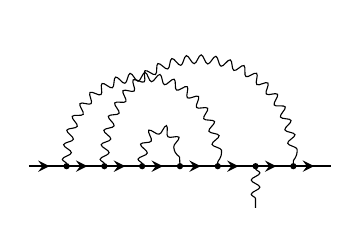
\begin{tikzpicture}[scale=0.48,baseline=(current bounding box.south)]
\draw[fermion] (0,0) -- (1,0);
\draw[fermion] (1,0) -- (2,0);
\draw[fermion] (2,0) -- (3,0);
\draw[fermion] (3,0) -- (4,0);
\draw[fermion] (4,0) -- (5,0);
\draw[fermion] (5,0) -- (6,0);
\draw[fermion] (6,0) -- (7,0);
\draw[fermion] (7,0) -- (8,0);
\draw[photon] (6,0) -- (6,-1.1);
\draw[photon] (1,0) .. controls (1,3.03) and (5,3.03) .. (5,0);
\draw[photon] (2,0) .. controls (2,3.65) and (7,3.65) .. (7,0);
\draw[photon] (3,0) .. controls (3,1.17) and (4,1.17) .. (4,0);
\node[vtx] at (1,0) {};
\node[vtx] at (2,0) {};
\node[vtx] at (3,0) {};
\node[vtx] at (4,0) {};
\node[vtx] at (5,0) {};
\node[vtx] at (6,0) {};
\node[vtx] at (7,0) {};
\end{tikzpicture}}{\texttt{g3\_06} mirror: 6; 1-5, 2-7, 3-4}\hfill\dcell{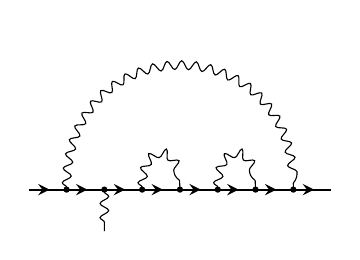
\begin{tikzpicture}[scale=0.48,baseline=(current bounding box.south)]
\draw[fermion] (0,0) -- (1,0);
\draw[fermion] (1,0) -- (2,0);
\draw[fermion] (2,0) -- (3,0);
\draw[fermion] (3,0) -- (4,0);
\draw[fermion] (4,0) -- (5,0);
\draw[fermion] (5,0) -- (6,0);
\draw[fermion] (6,0) -- (7,0);
\draw[fermion] (7,0) -- (8,0);
\draw[photon] (2,0) -- (2,-1.1);
\draw[photon] (1,0) .. controls (1,4.27) and (7,4.27) .. (7,0);
\draw[photon] (3,0) .. controls (3,1.17) and (4,1.17) .. (4,0);
\draw[photon] (5,0) .. controls (5,1.17) and (6,1.17) .. (6,0);
\node[vtx] at (1,0) {};
\node[vtx] at (2,0) {};
\node[vtx] at (3,0) {};
\node[vtx] at (4,0) {};
\node[vtx] at (5,0) {};
\node[vtx] at (6,0) {};
\node[vtx] at (7,0) {};
\end{tikzpicture}}{\texttt{g3\_07}\ \ 2; 1-7, 3-4, 5-6\ \ [2]}\hfill\dcell{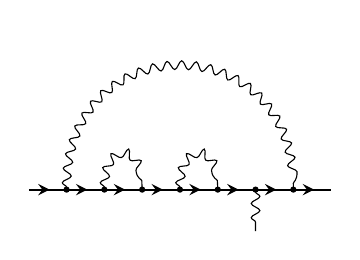
\begin{tikzpicture}[scale=0.48,baseline=(current bounding box.south)]
\draw[fermion] (0,0) -- (1,0);
\draw[fermion] (1,0) -- (2,0);
\draw[fermion] (2,0) -- (3,0);
\draw[fermion] (3,0) -- (4,0);
\draw[fermion] (4,0) -- (5,0);
\draw[fermion] (5,0) -- (6,0);
\draw[fermion] (6,0) -- (7,0);
\draw[fermion] (7,0) -- (8,0);
\draw[photon] (6,0) -- (6,-1.1);
\draw[photon] (1,0) .. controls (1,4.27) and (7,4.27) .. (7,0);
\draw[photon] (2,0) .. controls (2,1.17) and (3,1.17) .. (3,0);
\draw[photon] (4,0) .. controls (4,1.17) and (5,1.17) .. (5,0);
\node[vtx] at (1,0) {};
\node[vtx] at (2,0) {};
\node[vtx] at (3,0) {};
\node[vtx] at (4,0) {};
\node[vtx] at (5,0) {};
\node[vtx] at (6,0) {};
\node[vtx] at (7,0) {};
\end{tikzpicture}}{\texttt{g3\_07} mirror: 6; 1-7, 2-3, 4-5}\hfill\mbox{}\par\vspace{3mm}
\dcell{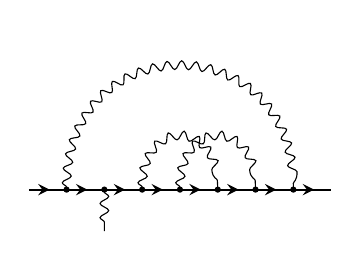
\begin{tikzpicture}[scale=0.48,baseline=(current bounding box.south)]
\draw[fermion] (0,0) -- (1,0);
\draw[fermion] (1,0) -- (2,0);
\draw[fermion] (2,0) -- (3,0);
\draw[fermion] (3,0) -- (4,0);
\draw[fermion] (4,0) -- (5,0);
\draw[fermion] (5,0) -- (6,0);
\draw[fermion] (6,0) -- (7,0);
\draw[fermion] (7,0) -- (8,0);
\draw[photon] (2,0) -- (2,-1.1);
\draw[photon] (1,0) .. controls (1,4.27) and (7,4.27) .. (7,0);
\draw[photon] (3,0) .. controls (3,1.79) and (5,1.79) .. (5,0);
\draw[photon] (4,0) .. controls (4,1.79) and (6,1.79) .. (6,0);
\node[vtx] at (1,0) {};
\node[vtx] at (2,0) {};
\node[vtx] at (3,0) {};
\node[vtx] at (4,0) {};
\node[vtx] at (5,0) {};
\node[vtx] at (6,0) {};
\node[vtx] at (7,0) {};
\end{tikzpicture}}{\texttt{g3\_08}\ \ 2; 1-7, 3-5, 4-6\ \ [2]}\hfill\dcell{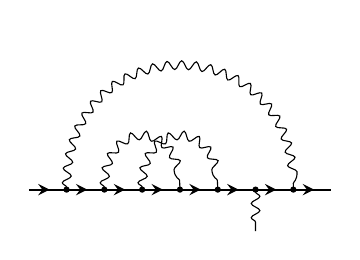
\begin{tikzpicture}[scale=0.48,baseline=(current bounding box.south)]
\draw[fermion] (0,0) -- (1,0);
\draw[fermion] (1,0) -- (2,0);
\draw[fermion] (2,0) -- (3,0);
\draw[fermion] (3,0) -- (4,0);
\draw[fermion] (4,0) -- (5,0);
\draw[fermion] (5,0) -- (6,0);
\draw[fermion] (6,0) -- (7,0);
\draw[fermion] (7,0) -- (8,0);
\draw[photon] (6,0) -- (6,-1.1);
\draw[photon] (1,0) .. controls (1,4.27) and (7,4.27) .. (7,0);
\draw[photon] (2,0) .. controls (2,1.79) and (4,1.79) .. (4,0);
\draw[photon] (3,0) .. controls (3,1.79) and (5,1.79) .. (5,0);
\node[vtx] at (1,0) {};
\node[vtx] at (2,0) {};
\node[vtx] at (3,0) {};
\node[vtx] at (4,0) {};
\node[vtx] at (5,0) {};
\node[vtx] at (6,0) {};
\node[vtx] at (7,0) {};
\end{tikzpicture}}{\texttt{g3\_08} mirror: 6; 1-7, 2-4, 3-5}\hfill\dcell{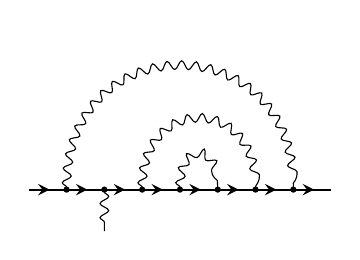
\begin{tikzpicture}[scale=0.48,baseline=(current bounding box.south)]
\draw[fermion] (0,0) -- (1,0);
\draw[fermion] (1,0) -- (2,0);
\draw[fermion] (2,0) -- (3,0);
\draw[fermion] (3,0) -- (4,0);
\draw[fermion] (4,0) -- (5,0);
\draw[fermion] (5,0) -- (6,0);
\draw[fermion] (6,0) -- (7,0);
\draw[fermion] (7,0) -- (8,0);
\draw[photon] (2,0) -- (2,-1.1);
\draw[photon] (1,0) .. controls (1,4.27) and (7,4.27) .. (7,0);
\draw[photon] (3,0) .. controls (3,2.41) and (6,2.41) .. (6,0);
\draw[photon] (4,0) .. controls (4,1.17) and (5,1.17) .. (5,0);
\node[vtx] at (1,0) {};
\node[vtx] at (2,0) {};
\node[vtx] at (3,0) {};
\node[vtx] at (4,0) {};
\node[vtx] at (5,0) {};
\node[vtx] at (6,0) {};
\node[vtx] at (7,0) {};
\end{tikzpicture}}{\texttt{g3\_09}\ \ 2; 1-7, 3-6, 4-5\ \ [2]}\hfill\dcell{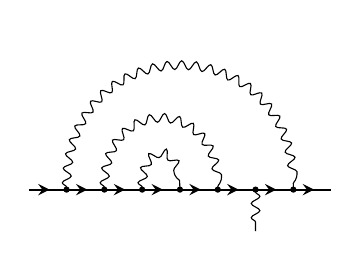
\begin{tikzpicture}[scale=0.48,baseline=(current bounding box.south)]
\draw[fermion] (0,0) -- (1,0);
\draw[fermion] (1,0) -- (2,0);
\draw[fermion] (2,0) -- (3,0);
\draw[fermion] (3,0) -- (4,0);
\draw[fermion] (4,0) -- (5,0);
\draw[fermion] (5,0) -- (6,0);
\draw[fermion] (6,0) -- (7,0);
\draw[fermion] (7,0) -- (8,0);
\draw[photon] (6,0) -- (6,-1.1);
\draw[photon] (1,0) .. controls (1,4.27) and (7,4.27) .. (7,0);
\draw[photon] (2,0) .. controls (2,2.41) and (5,2.41) .. (5,0);
\draw[photon] (3,0) .. controls (3,1.17) and (4,1.17) .. (4,0);
\node[vtx] at (1,0) {};
\node[vtx] at (2,0) {};
\node[vtx] at (3,0) {};
\node[vtx] at (4,0) {};
\node[vtx] at (5,0) {};
\node[vtx] at (6,0) {};
\node[vtx] at (7,0) {};
\end{tikzpicture}}{\texttt{g3\_09} mirror: 6; 1-7, 2-5, 3-4}\hfill\mbox{}\par\vspace{3mm}
\dcell{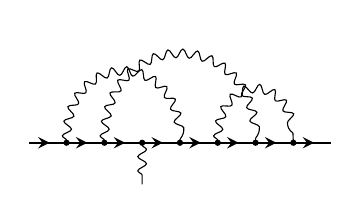
\begin{tikzpicture}[scale=0.48,baseline=(current bounding box.south)]
\draw[fermion] (0,0) -- (1,0);
\draw[fermion] (1,0) -- (2,0);
\draw[fermion] (2,0) -- (3,0);
\draw[fermion] (3,0) -- (4,0);
\draw[fermion] (4,0) -- (5,0);
\draw[fermion] (5,0) -- (6,0);
\draw[fermion] (6,0) -- (7,0);
\draw[fermion] (7,0) -- (8,0);
\draw[photon] (3,0) -- (3,-1.1);
\draw[photon] (1,0) .. controls (1,2.41) and (4,2.41) .. (4,0);
\draw[photon] (2,0) .. controls (2,3.03) and (6,3.03) .. (6,0);
\draw[photon] (5,0) .. controls (5,1.79) and (7,1.79) .. (7,0);
\node[vtx] at (1,0) {};
\node[vtx] at (2,0) {};
\node[vtx] at (3,0) {};
\node[vtx] at (4,0) {};
\node[vtx] at (5,0) {};
\node[vtx] at (6,0) {};
\node[vtx] at (7,0) {};
\end{tikzpicture}}{\texttt{g3\_10}\ \ 3; 1-4, 2-6, 5-7\ \ [2]}\hfill\dcell{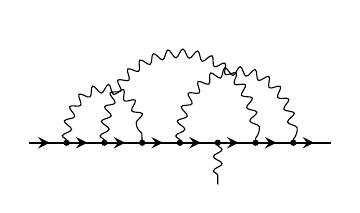
\begin{tikzpicture}[scale=0.48,baseline=(current bounding box.south)]
\draw[fermion] (0,0) -- (1,0);
\draw[fermion] (1,0) -- (2,0);
\draw[fermion] (2,0) -- (3,0);
\draw[fermion] (3,0) -- (4,0);
\draw[fermion] (4,0) -- (5,0);
\draw[fermion] (5,0) -- (6,0);
\draw[fermion] (6,0) -- (7,0);
\draw[fermion] (7,0) -- (8,0);
\draw[photon] (5,0) -- (5,-1.1);
\draw[photon] (1,0) .. controls (1,1.79) and (3,1.79) .. (3,0);
\draw[photon] (2,0) .. controls (2,3.03) and (6,3.03) .. (6,0);
\draw[photon] (4,0) .. controls (4,2.41) and (7,2.41) .. (7,0);
\node[vtx] at (1,0) {};
\node[vtx] at (2,0) {};
\node[vtx] at (3,0) {};
\node[vtx] at (4,0) {};
\node[vtx] at (5,0) {};
\node[vtx] at (6,0) {};
\node[vtx] at (7,0) {};
\end{tikzpicture}}{\texttt{g3\_10} mirror: 5; 1-3, 2-6, 4-7}\hfill\dcell{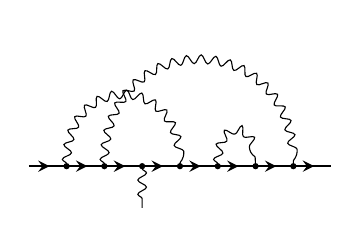
\begin{tikzpicture}[scale=0.48,baseline=(current bounding box.south)]
\draw[fermion] (0,0) -- (1,0);
\draw[fermion] (1,0) -- (2,0);
\draw[fermion] (2,0) -- (3,0);
\draw[fermion] (3,0) -- (4,0);
\draw[fermion] (4,0) -- (5,0);
\draw[fermion] (5,0) -- (6,0);
\draw[fermion] (6,0) -- (7,0);
\draw[fermion] (7,0) -- (8,0);
\draw[photon] (3,0) -- (3,-1.1);
\draw[photon] (1,0) .. controls (1,2.41) and (4,2.41) .. (4,0);
\draw[photon] (2,0) .. controls (2,3.65) and (7,3.65) .. (7,0);
\draw[photon] (5,0) .. controls (5,1.17) and (6,1.17) .. (6,0);
\node[vtx] at (1,0) {};
\node[vtx] at (2,0) {};
\node[vtx] at (3,0) {};
\node[vtx] at (4,0) {};
\node[vtx] at (5,0) {};
\node[vtx] at (6,0) {};
\node[vtx] at (7,0) {};
\end{tikzpicture}}{\texttt{g3\_11}\ \ 3; 1-4, 2-7, 5-6\ \ [2]}\hfill\dcell{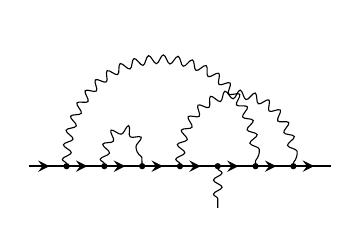
\begin{tikzpicture}[scale=0.48,baseline=(current bounding box.south)]
\draw[fermion] (0,0) -- (1,0);
\draw[fermion] (1,0) -- (2,0);
\draw[fermion] (2,0) -- (3,0);
\draw[fermion] (3,0) -- (4,0);
\draw[fermion] (4,0) -- (5,0);
\draw[fermion] (5,0) -- (6,0);
\draw[fermion] (6,0) -- (7,0);
\draw[fermion] (7,0) -- (8,0);
\draw[photon] (5,0) -- (5,-1.1);
\draw[photon] (1,0) .. controls (1,3.65) and (6,3.65) .. (6,0);
\draw[photon] (2,0) .. controls (2,1.17) and (3,1.17) .. (3,0);
\draw[photon] (4,0) .. controls (4,2.41) and (7,2.41) .. (7,0);
\node[vtx] at (1,0) {};
\node[vtx] at (2,0) {};
\node[vtx] at (3,0) {};
\node[vtx] at (4,0) {};
\node[vtx] at (5,0) {};
\node[vtx] at (6,0) {};
\node[vtx] at (7,0) {};
\end{tikzpicture}}{\texttt{g3\_11} mirror: 5; 1-6, 2-3, 4-7}\hfill\mbox{}\par\vspace{3mm}
\dcell{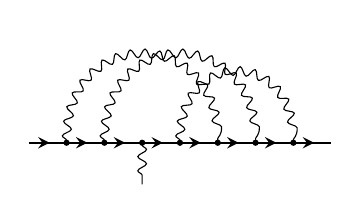
\begin{tikzpicture}[scale=0.48,baseline=(current bounding box.south)]
\draw[fermion] (0,0) -- (1,0);
\draw[fermion] (1,0) -- (2,0);
\draw[fermion] (2,0) -- (3,0);
\draw[fermion] (3,0) -- (4,0);
\draw[fermion] (4,0) -- (5,0);
\draw[fermion] (5,0) -- (6,0);
\draw[fermion] (6,0) -- (7,0);
\draw[fermion] (7,0) -- (8,0);
\draw[photon] (3,0) -- (3,-1.1);
\draw[photon] (1,0) .. controls (1,3.03) and (5,3.03) .. (5,0);
\draw[photon] (2,0) .. controls (2,3.03) and (6,3.03) .. (6,0);
\draw[photon] (4,0) .. controls (4,2.41) and (7,2.41) .. (7,0);
\node[vtx] at (1,0) {};
\node[vtx] at (2,0) {};
\node[vtx] at (3,0) {};
\node[vtx] at (4,0) {};
\node[vtx] at (5,0) {};
\node[vtx] at (6,0) {};
\node[vtx] at (7,0) {};
\end{tikzpicture}}{\texttt{g3\_12}\ \ 3; 1-5, 2-6, 4-7\ \ [2]}\hfill\dcell{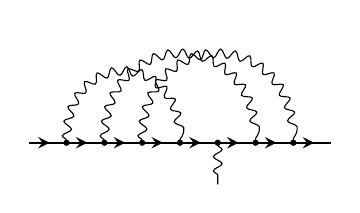
\begin{tikzpicture}[scale=0.48,baseline=(current bounding box.south)]
\draw[fermion] (0,0) -- (1,0);
\draw[fermion] (1,0) -- (2,0);
\draw[fermion] (2,0) -- (3,0);
\draw[fermion] (3,0) -- (4,0);
\draw[fermion] (4,0) -- (5,0);
\draw[fermion] (5,0) -- (6,0);
\draw[fermion] (6,0) -- (7,0);
\draw[fermion] (7,0) -- (8,0);
\draw[photon] (5,0) -- (5,-1.1);
\draw[photon] (1,0) .. controls (1,2.41) and (4,2.41) .. (4,0);
\draw[photon] (2,0) .. controls (2,3.03) and (6,3.03) .. (6,0);
\draw[photon] (3,0) .. controls (3,3.03) and (7,3.03) .. (7,0);
\node[vtx] at (1,0) {};
\node[vtx] at (2,0) {};
\node[vtx] at (3,0) {};
\node[vtx] at (4,0) {};
\node[vtx] at (5,0) {};
\node[vtx] at (6,0) {};
\node[vtx] at (7,0) {};
\end{tikzpicture}}{\texttt{g3\_12} mirror: 5; 1-4, 2-6, 3-7}\hfill\dcell{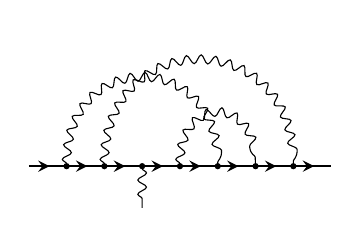
\begin{tikzpicture}[scale=0.48,baseline=(current bounding box.south)]
\draw[fermion] (0,0) -- (1,0);
\draw[fermion] (1,0) -- (2,0);
\draw[fermion] (2,0) -- (3,0);
\draw[fermion] (3,0) -- (4,0);
\draw[fermion] (4,0) -- (5,0);
\draw[fermion] (5,0) -- (6,0);
\draw[fermion] (6,0) -- (7,0);
\draw[fermion] (7,0) -- (8,0);
\draw[photon] (3,0) -- (3,-1.1);
\draw[photon] (1,0) .. controls (1,3.03) and (5,3.03) .. (5,0);
\draw[photon] (2,0) .. controls (2,3.65) and (7,3.65) .. (7,0);
\draw[photon] (4,0) .. controls (4,1.79) and (6,1.79) .. (6,0);
\node[vtx] at (1,0) {};
\node[vtx] at (2,0) {};
\node[vtx] at (3,0) {};
\node[vtx] at (4,0) {};
\node[vtx] at (5,0) {};
\node[vtx] at (6,0) {};
\node[vtx] at (7,0) {};
\end{tikzpicture}}{\texttt{g3\_13}\ \ 3; 1-5, 2-7, 4-6\ \ [2]}\hfill\dcell{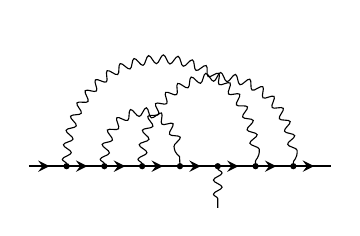
\begin{tikzpicture}[scale=0.48,baseline=(current bounding box.south)]
\draw[fermion] (0,0) -- (1,0);
\draw[fermion] (1,0) -- (2,0);
\draw[fermion] (2,0) -- (3,0);
\draw[fermion] (3,0) -- (4,0);
\draw[fermion] (4,0) -- (5,0);
\draw[fermion] (5,0) -- (6,0);
\draw[fermion] (6,0) -- (7,0);
\draw[fermion] (7,0) -- (8,0);
\draw[photon] (5,0) -- (5,-1.1);
\draw[photon] (1,0) .. controls (1,3.65) and (6,3.65) .. (6,0);
\draw[photon] (2,0) .. controls (2,1.79) and (4,1.79) .. (4,0);
\draw[photon] (3,0) .. controls (3,3.03) and (7,3.03) .. (7,0);
\node[vtx] at (1,0) {};
\node[vtx] at (2,0) {};
\node[vtx] at (3,0) {};
\node[vtx] at (4,0) {};
\node[vtx] at (5,0) {};
\node[vtx] at (6,0) {};
\node[vtx] at (7,0) {};
\end{tikzpicture}}{\texttt{g3\_13} mirror: 5; 1-6, 2-4, 3-7}\hfill\mbox{}\par\vspace{3mm}
\dcell{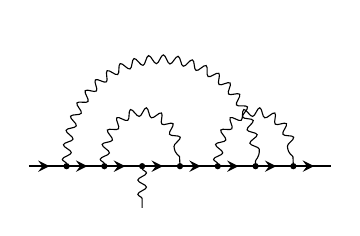
\begin{tikzpicture}[scale=0.48,baseline=(current bounding box.south)]
\draw[fermion] (0,0) -- (1,0);
\draw[fermion] (1,0) -- (2,0);
\draw[fermion] (2,0) -- (3,0);
\draw[fermion] (3,0) -- (4,0);
\draw[fermion] (4,0) -- (5,0);
\draw[fermion] (5,0) -- (6,0);
\draw[fermion] (6,0) -- (7,0);
\draw[fermion] (7,0) -- (8,0);
\draw[photon] (3,0) -- (3,-1.1);
\draw[photon] (1,0) .. controls (1,3.65) and (6,3.65) .. (6,0);
\draw[photon] (2,0) .. controls (2,1.79) and (4,1.79) .. (4,0);
\draw[photon] (5,0) .. controls (5,1.79) and (7,1.79) .. (7,0);
\node[vtx] at (1,0) {};
\node[vtx] at (2,0) {};
\node[vtx] at (3,0) {};
\node[vtx] at (4,0) {};
\node[vtx] at (5,0) {};
\node[vtx] at (6,0) {};
\node[vtx] at (7,0) {};
\end{tikzpicture}}{\texttt{g3\_14}\ \ 3; 1-6, 2-4, 5-7\ \ [2]}\hfill\dcell{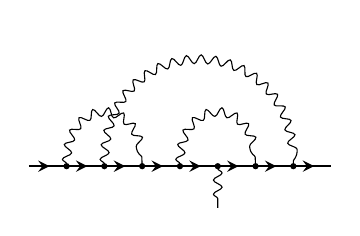
\begin{tikzpicture}[scale=0.48,baseline=(current bounding box.south)]
\draw[fermion] (0,0) -- (1,0);
\draw[fermion] (1,0) -- (2,0);
\draw[fermion] (2,0) -- (3,0);
\draw[fermion] (3,0) -- (4,0);
\draw[fermion] (4,0) -- (5,0);
\draw[fermion] (5,0) -- (6,0);
\draw[fermion] (6,0) -- (7,0);
\draw[fermion] (7,0) -- (8,0);
\draw[photon] (5,0) -- (5,-1.1);
\draw[photon] (1,0) .. controls (1,1.79) and (3,1.79) .. (3,0);
\draw[photon] (2,0) .. controls (2,3.65) and (7,3.65) .. (7,0);
\draw[photon] (4,0) .. controls (4,1.79) and (6,1.79) .. (6,0);
\node[vtx] at (1,0) {};
\node[vtx] at (2,0) {};
\node[vtx] at (3,0) {};
\node[vtx] at (4,0) {};
\node[vtx] at (5,0) {};
\node[vtx] at (6,0) {};
\node[vtx] at (7,0) {};
\end{tikzpicture}}{\texttt{g3\_14} mirror: 5; 1-3, 2-7, 4-6}\hfill\dcell{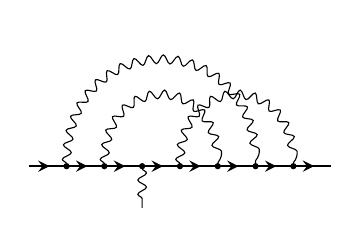
\begin{tikzpicture}[scale=0.48,baseline=(current bounding box.south)]
\draw[fermion] (0,0) -- (1,0);
\draw[fermion] (1,0) -- (2,0);
\draw[fermion] (2,0) -- (3,0);
\draw[fermion] (3,0) -- (4,0);
\draw[fermion] (4,0) -- (5,0);
\draw[fermion] (5,0) -- (6,0);
\draw[fermion] (6,0) -- (7,0);
\draw[fermion] (7,0) -- (8,0);
\draw[photon] (3,0) -- (3,-1.1);
\draw[photon] (1,0) .. controls (1,3.65) and (6,3.65) .. (6,0);
\draw[photon] (2,0) .. controls (2,2.41) and (5,2.41) .. (5,0);
\draw[photon] (4,0) .. controls (4,2.41) and (7,2.41) .. (7,0);
\node[vtx] at (1,0) {};
\node[vtx] at (2,0) {};
\node[vtx] at (3,0) {};
\node[vtx] at (4,0) {};
\node[vtx] at (5,0) {};
\node[vtx] at (6,0) {};
\node[vtx] at (7,0) {};
\end{tikzpicture}}{\texttt{g3\_15}\ \ 3; 1-6, 2-5, 4-7\ \ [2]}\hfill\dcell{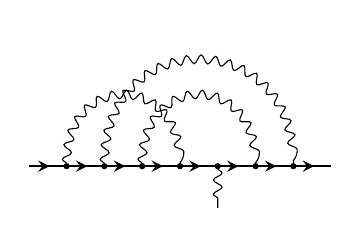
\begin{tikzpicture}[scale=0.48,baseline=(current bounding box.south)]
\draw[fermion] (0,0) -- (1,0);
\draw[fermion] (1,0) -- (2,0);
\draw[fermion] (2,0) -- (3,0);
\draw[fermion] (3,0) -- (4,0);
\draw[fermion] (4,0) -- (5,0);
\draw[fermion] (5,0) -- (6,0);
\draw[fermion] (6,0) -- (7,0);
\draw[fermion] (7,0) -- (8,0);
\draw[photon] (5,0) -- (5,-1.1);
\draw[photon] (1,0) .. controls (1,2.41) and (4,2.41) .. (4,0);
\draw[photon] (2,0) .. controls (2,3.65) and (7,3.65) .. (7,0);
\draw[photon] (3,0) .. controls (3,2.41) and (6,2.41) .. (6,0);
\node[vtx] at (1,0) {};
\node[vtx] at (2,0) {};
\node[vtx] at (3,0) {};
\node[vtx] at (4,0) {};
\node[vtx] at (5,0) {};
\node[vtx] at (6,0) {};
\node[vtx] at (7,0) {};
\end{tikzpicture}}{\texttt{g3\_15} mirror: 5; 1-4, 2-7, 3-6}\hfill\mbox{}\par\vspace{3mm}
\dcell{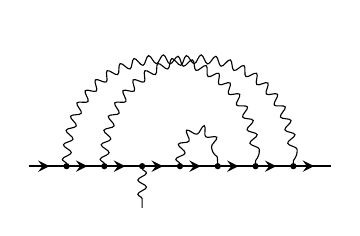
\begin{tikzpicture}[scale=0.48,baseline=(current bounding box.south)]
\draw[fermion] (0,0) -- (1,0);
\draw[fermion] (1,0) -- (2,0);
\draw[fermion] (2,0) -- (3,0);
\draw[fermion] (3,0) -- (4,0);
\draw[fermion] (4,0) -- (5,0);
\draw[fermion] (5,0) -- (6,0);
\draw[fermion] (6,0) -- (7,0);
\draw[fermion] (7,0) -- (8,0);
\draw[photon] (3,0) -- (3,-1.1);
\draw[photon] (1,0) .. controls (1,3.65) and (6,3.65) .. (6,0);
\draw[photon] (2,0) .. controls (2,3.65) and (7,3.65) .. (7,0);
\draw[photon] (4,0) .. controls (4,1.17) and (5,1.17) .. (5,0);
\node[vtx] at (1,0) {};
\node[vtx] at (2,0) {};
\node[vtx] at (3,0) {};
\node[vtx] at (4,0) {};
\node[vtx] at (5,0) {};
\node[vtx] at (6,0) {};
\node[vtx] at (7,0) {};
\end{tikzpicture}}{\texttt{g3\_16}\ \ 3; 1-6, 2-7, 4-5\ \ [2]}\hfill\dcell{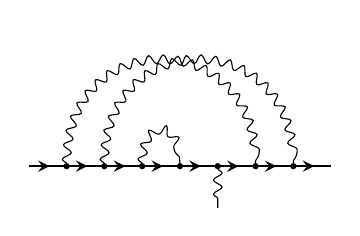
\begin{tikzpicture}[scale=0.48,baseline=(current bounding box.south)]
\draw[fermion] (0,0) -- (1,0);
\draw[fermion] (1,0) -- (2,0);
\draw[fermion] (2,0) -- (3,0);
\draw[fermion] (3,0) -- (4,0);
\draw[fermion] (4,0) -- (5,0);
\draw[fermion] (5,0) -- (6,0);
\draw[fermion] (6,0) -- (7,0);
\draw[fermion] (7,0) -- (8,0);
\draw[photon] (5,0) -- (5,-1.1);
\draw[photon] (1,0) .. controls (1,3.65) and (6,3.65) .. (6,0);
\draw[photon] (2,0) .. controls (2,3.65) and (7,3.65) .. (7,0);
\draw[photon] (3,0) .. controls (3,1.17) and (4,1.17) .. (4,0);
\node[vtx] at (1,0) {};
\node[vtx] at (2,0) {};
\node[vtx] at (3,0) {};
\node[vtx] at (4,0) {};
\node[vtx] at (5,0) {};
\node[vtx] at (6,0) {};
\node[vtx] at (7,0) {};
\end{tikzpicture}}{\texttt{g3\_16} mirror: 5; 1-6, 2-7, 3-4}\hfill\dcell{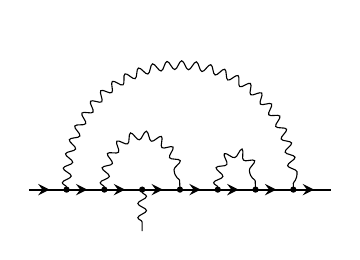
\begin{tikzpicture}[scale=0.48,baseline=(current bounding box.south)]
\draw[fermion] (0,0) -- (1,0);
\draw[fermion] (1,0) -- (2,0);
\draw[fermion] (2,0) -- (3,0);
\draw[fermion] (3,0) -- (4,0);
\draw[fermion] (4,0) -- (5,0);
\draw[fermion] (5,0) -- (6,0);
\draw[fermion] (6,0) -- (7,0);
\draw[fermion] (7,0) -- (8,0);
\draw[photon] (3,0) -- (3,-1.1);
\draw[photon] (1,0) .. controls (1,4.27) and (7,4.27) .. (7,0);
\draw[photon] (2,0) .. controls (2,1.79) and (4,1.79) .. (4,0);
\draw[photon] (5,0) .. controls (5,1.17) and (6,1.17) .. (6,0);
\node[vtx] at (1,0) {};
\node[vtx] at (2,0) {};
\node[vtx] at (3,0) {};
\node[vtx] at (4,0) {};
\node[vtx] at (5,0) {};
\node[vtx] at (6,0) {};
\node[vtx] at (7,0) {};
\end{tikzpicture}}{\texttt{g3\_17}\ \ 3; 1-7, 2-4, 5-6\ \ [2]}\hfill\dcell{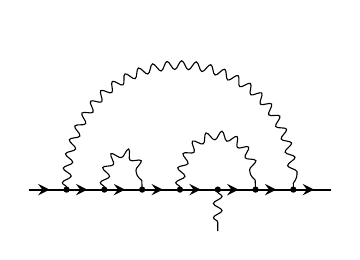
\begin{tikzpicture}[scale=0.48,baseline=(current bounding box.south)]
\draw[fermion] (0,0) -- (1,0);
\draw[fermion] (1,0) -- (2,0);
\draw[fermion] (2,0) -- (3,0);
\draw[fermion] (3,0) -- (4,0);
\draw[fermion] (4,0) -- (5,0);
\draw[fermion] (5,0) -- (6,0);
\draw[fermion] (6,0) -- (7,0);
\draw[fermion] (7,0) -- (8,0);
\draw[photon] (5,0) -- (5,-1.1);
\draw[photon] (1,0) .. controls (1,4.27) and (7,4.27) .. (7,0);
\draw[photon] (2,0) .. controls (2,1.17) and (3,1.17) .. (3,0);
\draw[photon] (4,0) .. controls (4,1.79) and (6,1.79) .. (6,0);
\node[vtx] at (1,0) {};
\node[vtx] at (2,0) {};
\node[vtx] at (3,0) {};
\node[vtx] at (4,0) {};
\node[vtx] at (5,0) {};
\node[vtx] at (6,0) {};
\node[vtx] at (7,0) {};
\end{tikzpicture}}{\texttt{g3\_17} mirror: 5; 1-7, 2-3, 4-6}\hfill\mbox{}\par\vspace{3mm}
\dcell{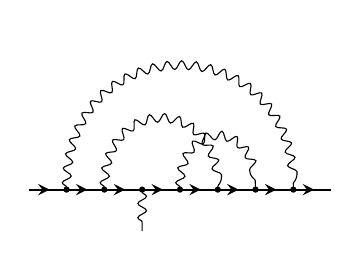
\begin{tikzpicture}[scale=0.48,baseline=(current bounding box.south)]
\draw[fermion] (0,0) -- (1,0);
\draw[fermion] (1,0) -- (2,0);
\draw[fermion] (2,0) -- (3,0);
\draw[fermion] (3,0) -- (4,0);
\draw[fermion] (4,0) -- (5,0);
\draw[fermion] (5,0) -- (6,0);
\draw[fermion] (6,0) -- (7,0);
\draw[fermion] (7,0) -- (8,0);
\draw[photon] (3,0) -- (3,-1.1);
\draw[photon] (1,0) .. controls (1,4.27) and (7,4.27) .. (7,0);
\draw[photon] (2,0) .. controls (2,2.41) and (5,2.41) .. (5,0);
\draw[photon] (4,0) .. controls (4,1.79) and (6,1.79) .. (6,0);
\node[vtx] at (1,0) {};
\node[vtx] at (2,0) {};
\node[vtx] at (3,0) {};
\node[vtx] at (4,0) {};
\node[vtx] at (5,0) {};
\node[vtx] at (6,0) {};
\node[vtx] at (7,0) {};
\end{tikzpicture}}{\texttt{g3\_18}\ \ 3; 1-7, 2-5, 4-6\ \ [2]}\hfill\dcell{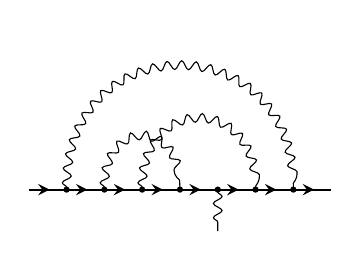
\begin{tikzpicture}[scale=0.48,baseline=(current bounding box.south)]
\draw[fermion] (0,0) -- (1,0);
\draw[fermion] (1,0) -- (2,0);
\draw[fermion] (2,0) -- (3,0);
\draw[fermion] (3,0) -- (4,0);
\draw[fermion] (4,0) -- (5,0);
\draw[fermion] (5,0) -- (6,0);
\draw[fermion] (6,0) -- (7,0);
\draw[fermion] (7,0) -- (8,0);
\draw[photon] (5,0) -- (5,-1.1);
\draw[photon] (1,0) .. controls (1,4.27) and (7,4.27) .. (7,0);
\draw[photon] (2,0) .. controls (2,1.79) and (4,1.79) .. (4,0);
\draw[photon] (3,0) .. controls (3,2.41) and (6,2.41) .. (6,0);
\node[vtx] at (1,0) {};
\node[vtx] at (2,0) {};
\node[vtx] at (3,0) {};
\node[vtx] at (4,0) {};
\node[vtx] at (5,0) {};
\node[vtx] at (6,0) {};
\node[vtx] at (7,0) {};
\end{tikzpicture}}{\texttt{g3\_18} mirror: 5; 1-7, 2-4, 3-6}\hfill\dcell{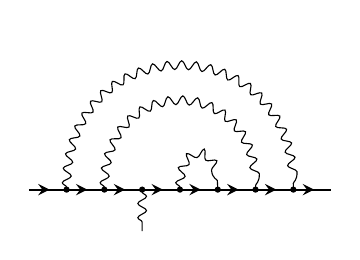
\begin{tikzpicture}[scale=0.48,baseline=(current bounding box.south)]
\draw[fermion] (0,0) -- (1,0);
\draw[fermion] (1,0) -- (2,0);
\draw[fermion] (2,0) -- (3,0);
\draw[fermion] (3,0) -- (4,0);
\draw[fermion] (4,0) -- (5,0);
\draw[fermion] (5,0) -- (6,0);
\draw[fermion] (6,0) -- (7,0);
\draw[fermion] (7,0) -- (8,0);
\draw[photon] (3,0) -- (3,-1.1);
\draw[photon] (1,0) .. controls (1,4.27) and (7,4.27) .. (7,0);
\draw[photon] (2,0) .. controls (2,3.03) and (6,3.03) .. (6,0);
\draw[photon] (4,0) .. controls (4,1.17) and (5,1.17) .. (5,0);
\node[vtx] at (1,0) {};
\node[vtx] at (2,0) {};
\node[vtx] at (3,0) {};
\node[vtx] at (4,0) {};
\node[vtx] at (5,0) {};
\node[vtx] at (6,0) {};
\node[vtx] at (7,0) {};
\end{tikzpicture}}{\texttt{g3\_19}\ \ 3; 1-7, 2-6, 4-5\ \ [2]}\hfill\dcell{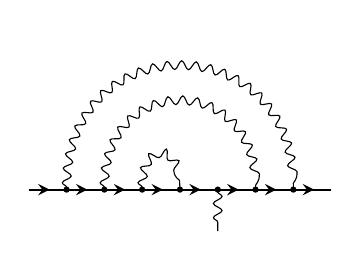
\begin{tikzpicture}[scale=0.48,baseline=(current bounding box.south)]
\draw[fermion] (0,0) -- (1,0);
\draw[fermion] (1,0) -- (2,0);
\draw[fermion] (2,0) -- (3,0);
\draw[fermion] (3,0) -- (4,0);
\draw[fermion] (4,0) -- (5,0);
\draw[fermion] (5,0) -- (6,0);
\draw[fermion] (6,0) -- (7,0);
\draw[fermion] (7,0) -- (8,0);
\draw[photon] (5,0) -- (5,-1.1);
\draw[photon] (1,0) .. controls (1,4.27) and (7,4.27) .. (7,0);
\draw[photon] (2,0) .. controls (2,3.03) and (6,3.03) .. (6,0);
\draw[photon] (3,0) .. controls (3,1.17) and (4,1.17) .. (4,0);
\node[vtx] at (1,0) {};
\node[vtx] at (2,0) {};
\node[vtx] at (3,0) {};
\node[vtx] at (4,0) {};
\node[vtx] at (5,0) {};
\node[vtx] at (6,0) {};
\node[vtx] at (7,0) {};
\end{tikzpicture}}{\texttt{g3\_19} mirror: 5; 1-7, 2-6, 3-4}\hfill\mbox{}\par\vspace{3mm}
\dcell{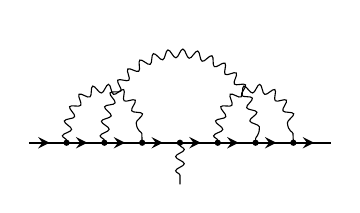
\begin{tikzpicture}[scale=0.48,baseline=(current bounding box.south)]
\draw[fermion] (0,0) -- (1,0);
\draw[fermion] (1,0) -- (2,0);
\draw[fermion] (2,0) -- (3,0);
\draw[fermion] (3,0) -- (4,0);
\draw[fermion] (4,0) -- (5,0);
\draw[fermion] (5,0) -- (6,0);
\draw[fermion] (6,0) -- (7,0);
\draw[fermion] (7,0) -- (8,0);
\draw[photon] (4,0) -- (4,-1.1);
\draw[photon] (1,0) .. controls (1,1.79) and (3,1.79) .. (3,0);
\draw[photon] (2,0) .. controls (2,3.03) and (6,3.03) .. (6,0);
\draw[photon] (5,0) .. controls (5,1.79) and (7,1.79) .. (7,0);
\node[vtx] at (1,0) {};
\node[vtx] at (2,0) {};
\node[vtx] at (3,0) {};
\node[vtx] at (4,0) {};
\node[vtx] at (5,0) {};
\node[vtx] at (6,0) {};
\node[vtx] at (7,0) {};
\end{tikzpicture}}{\texttt{g3\_20}\ \ 4; 1-3, 2-6, 5-7\ \ [1]}\hfill\dcell{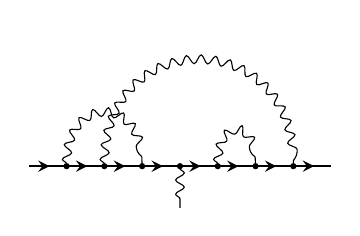
\begin{tikzpicture}[scale=0.48,baseline=(current bounding box.south)]
\draw[fermion] (0,0) -- (1,0);
\draw[fermion] (1,0) -- (2,0);
\draw[fermion] (2,0) -- (3,0);
\draw[fermion] (3,0) -- (4,0);
\draw[fermion] (4,0) -- (5,0);
\draw[fermion] (5,0) -- (6,0);
\draw[fermion] (6,0) -- (7,0);
\draw[fermion] (7,0) -- (8,0);
\draw[photon] (4,0) -- (4,-1.1);
\draw[photon] (1,0) .. controls (1,1.79) and (3,1.79) .. (3,0);
\draw[photon] (2,0) .. controls (2,3.65) and (7,3.65) .. (7,0);
\draw[photon] (5,0) .. controls (5,1.17) and (6,1.17) .. (6,0);
\node[vtx] at (1,0) {};
\node[vtx] at (2,0) {};
\node[vtx] at (3,0) {};
\node[vtx] at (4,0) {};
\node[vtx] at (5,0) {};
\node[vtx] at (6,0) {};
\node[vtx] at (7,0) {};
\end{tikzpicture}}{\texttt{g3\_21}\ \ 4; 1-3, 2-7, 5-6\ \ [2]}\hfill\dcell{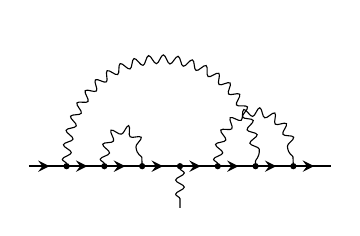
\begin{tikzpicture}[scale=0.48,baseline=(current bounding box.south)]
\draw[fermion] (0,0) -- (1,0);
\draw[fermion] (1,0) -- (2,0);
\draw[fermion] (2,0) -- (3,0);
\draw[fermion] (3,0) -- (4,0);
\draw[fermion] (4,0) -- (5,0);
\draw[fermion] (5,0) -- (6,0);
\draw[fermion] (6,0) -- (7,0);
\draw[fermion] (7,0) -- (8,0);
\draw[photon] (4,0) -- (4,-1.1);
\draw[photon] (1,0) .. controls (1,3.65) and (6,3.65) .. (6,0);
\draw[photon] (2,0) .. controls (2,1.17) and (3,1.17) .. (3,0);
\draw[photon] (5,0) .. controls (5,1.79) and (7,1.79) .. (7,0);
\node[vtx] at (1,0) {};
\node[vtx] at (2,0) {};
\node[vtx] at (3,0) {};
\node[vtx] at (4,0) {};
\node[vtx] at (5,0) {};
\node[vtx] at (6,0) {};
\node[vtx] at (7,0) {};
\end{tikzpicture}}{\texttt{g3\_21} mirror: 4; 1-6, 2-3, 5-7}\hfill\dcell{\begin{tikzpicture}[scale=0.48,baseline=(current bounding box.south)]
\draw[fermion] (0,0) -- (1,0);
\draw[fermion] (1,0) -- (2,0);
\draw[fermion] (2,0) -- (3,0);
\draw[fermion] (3,0) -- (4,0);
\draw[fermion] (4,0) -- (5,0);
\draw[fermion] (5,0) -- (6,0);
\draw[fermion] (6,0) -- (7,0);
\draw[fermion] (7,0) -- (8,0);
\draw[photon] (4,0) -- (4,-1.1);
\draw[photon] (1,0) .. controls (1,3.03) and (5,3.03) .. (5,0);
\draw[photon] (2,0) .. controls (2,3.03) and (6,3.03) .. (6,0);
\draw[photon] (3,0) .. controls (3,3.03) and (7,3.03) .. (7,0);
\node[vtx] at (1,0) {};
\node[vtx] at (2,0) {};
\node[vtx] at (3,0) {};
\node[vtx] at (4,0) {};
\node[vtx] at (5,0) {};
\node[vtx] at (6,0) {};
\node[vtx] at (7,0) {};
\end{tikzpicture}}{\texttt{g3\_22}\ \ 4; 1-5, 2-6, 3-7\ \ [1]}\hfill\mbox{}\par\vspace{3mm}
\dcell{\begin{tikzpicture}[scale=0.48,baseline=(current bounding box.south)]
\draw[fermion] (0,0) -- (1,0);
\draw[fermion] (1,0) -- (2,0);
\draw[fermion] (2,0) -- (3,0);
\draw[fermion] (3,0) -- (4,0);
\draw[fermion] (4,0) -- (5,0);
\draw[fermion] (5,0) -- (6,0);
\draw[fermion] (6,0) -- (7,0);
\draw[fermion] (7,0) -- (8,0);
\draw[photon] (4,0) -- (4,-1.1);
\draw[photon] (1,0) .. controls (1,3.03) and (5,3.03) .. (5,0);
\draw[photon] (2,0) .. controls (2,3.65) and (7,3.65) .. (7,0);
\draw[photon] (3,0) .. controls (3,2.41) and (6,2.41) .. (6,0);
\node[vtx] at (1,0) {};
\node[vtx] at (2,0) {};
\node[vtx] at (3,0) {};
\node[vtx] at (4,0) {};
\node[vtx] at (5,0) {};
\node[vtx] at (6,0) {};
\node[vtx] at (7,0) {};
\end{tikzpicture}}{\texttt{g3\_23}\ \ 4; 1-5, 2-7, 3-6\ \ [2]}\hfill\dcell{\begin{tikzpicture}[scale=0.48,baseline=(current bounding box.south)]
\draw[fermion] (0,0) -- (1,0);
\draw[fermion] (1,0) -- (2,0);
\draw[fermion] (2,0) -- (3,0);
\draw[fermion] (3,0) -- (4,0);
\draw[fermion] (4,0) -- (5,0);
\draw[fermion] (5,0) -- (6,0);
\draw[fermion] (6,0) -- (7,0);
\draw[fermion] (7,0) -- (8,0);
\draw[photon] (4,0) -- (4,-1.1);
\draw[photon] (1,0) .. controls (1,3.65) and (6,3.65) .. (6,0);
\draw[photon] (2,0) .. controls (2,2.41) and (5,2.41) .. (5,0);
\draw[photon] (3,0) .. controls (3,3.03) and (7,3.03) .. (7,0);
\node[vtx] at (1,0) {};
\node[vtx] at (2,0) {};
\node[vtx] at (3,0) {};
\node[vtx] at (4,0) {};
\node[vtx] at (5,0) {};
\node[vtx] at (6,0) {};
\node[vtx] at (7,0) {};
\end{tikzpicture}}{\texttt{g3\_23} mirror: 4; 1-6, 2-5, 3-7}\hfill\dcell{\begin{tikzpicture}[scale=0.48,baseline=(current bounding box.south)]
\draw[fermion] (0,0) -- (1,0);
\draw[fermion] (1,0) -- (2,0);
\draw[fermion] (2,0) -- (3,0);
\draw[fermion] (3,0) -- (4,0);
\draw[fermion] (4,0) -- (5,0);
\draw[fermion] (5,0) -- (6,0);
\draw[fermion] (6,0) -- (7,0);
\draw[fermion] (7,0) -- (8,0);
\draw[photon] (4,0) -- (4,-1.1);
\draw[photon] (1,0) .. controls (1,3.65) and (6,3.65) .. (6,0);
\draw[photon] (2,0) .. controls (2,3.65) and (7,3.65) .. (7,0);
\draw[photon] (3,0) .. controls (3,1.79) and (5,1.79) .. (5,0);
\node[vtx] at (1,0) {};
\node[vtx] at (2,0) {};
\node[vtx] at (3,0) {};
\node[vtx] at (4,0) {};
\node[vtx] at (5,0) {};
\node[vtx] at (6,0) {};
\node[vtx] at (7,0) {};
\end{tikzpicture}}{\texttt{g3\_24}\ \ 4; 1-6, 2-7, 3-5\ \ [1]}\hfill\dcell{\begin{tikzpicture}[scale=0.48,baseline=(current bounding box.south)]
\draw[fermion] (0,0) -- (1,0);
\draw[fermion] (1,0) -- (2,0);
\draw[fermion] (2,0) -- (3,0);
\draw[fermion] (3,0) -- (4,0);
\draw[fermion] (4,0) -- (5,0);
\draw[fermion] (5,0) -- (6,0);
\draw[fermion] (6,0) -- (7,0);
\draw[fermion] (7,0) -- (8,0);
\draw[photon] (4,0) -- (4,-1.1);
\draw[photon] (1,0) .. controls (1,4.27) and (7,4.27) .. (7,0);
\draw[photon] (2,0) .. controls (2,1.17) and (3,1.17) .. (3,0);
\draw[photon] (5,0) .. controls (5,1.17) and (6,1.17) .. (6,0);
\node[vtx] at (1,0) {};
\node[vtx] at (2,0) {};
\node[vtx] at (3,0) {};
\node[vtx] at (4,0) {};
\node[vtx] at (5,0) {};
\node[vtx] at (6,0) {};
\node[vtx] at (7,0) {};
\end{tikzpicture}}{\texttt{g3\_25}\ \ 4; 1-7, 2-3, 5-6\ \ [1]}\hfill\mbox{}\par\vspace{3mm}
\dcell{\begin{tikzpicture}[scale=0.48,baseline=(current bounding box.south)]
\draw[fermion] (0,0) -- (1,0);
\draw[fermion] (1,0) -- (2,0);
\draw[fermion] (2,0) -- (3,0);
\draw[fermion] (3,0) -- (4,0);
\draw[fermion] (4,0) -- (5,0);
\draw[fermion] (5,0) -- (6,0);
\draw[fermion] (6,0) -- (7,0);
\draw[fermion] (7,0) -- (8,0);
\draw[photon] (4,0) -- (4,-1.1);
\draw[photon] (1,0) .. controls (1,4.27) and (7,4.27) .. (7,0);
\draw[photon] (2,0) .. controls (2,2.41) and (5,2.41) .. (5,0);
\draw[photon] (3,0) .. controls (3,2.41) and (6,2.41) .. (6,0);
\node[vtx] at (1,0) {};
\node[vtx] at (2,0) {};
\node[vtx] at (3,0) {};
\node[vtx] at (4,0) {};
\node[vtx] at (5,0) {};
\node[vtx] at (6,0) {};
\node[vtx] at (7,0) {};
\end{tikzpicture}}{\texttt{g3\_26}\ \ 4; 1-7, 2-5, 3-6\ \ [1]}\hfill\dcell{\begin{tikzpicture}[scale=0.48,baseline=(current bounding box.south)]
\draw[fermion] (0,0) -- (1,0);
\draw[fermion] (1,0) -- (2,0);
\draw[fermion] (2,0) -- (3,0);
\draw[fermion] (3,0) -- (4,0);
\draw[fermion] (4,0) -- (5,0);
\draw[fermion] (5,0) -- (6,0);
\draw[fermion] (6,0) -- (7,0);
\draw[fermion] (7,0) -- (8,0);
\draw[photon] (4,0) -- (4,-1.1);
\draw[photon] (1,0) .. controls (1,4.27) and (7,4.27) .. (7,0);
\draw[photon] (2,0) .. controls (2,3.03) and (6,3.03) .. (6,0);
\draw[photon] (3,0) .. controls (3,1.79) and (5,1.79) .. (5,0);
\node[vtx] at (1,0) {};
\node[vtx] at (2,0) {};
\node[vtx] at (3,0) {};
\node[vtx] at (4,0) {};
\node[vtx] at (5,0) {};
\node[vtx] at (6,0) {};
\node[vtx] at (7,0) {};
\end{tikzpicture}}{\texttt{g3\_27}\ \ 4; 1-7, 2-6, 3-5\ \ [1]}\hfill\mbox{}\par\vspace{3mm}
\subsection*{Three loops with vacuum-polarization insertions (16 diagrams, group \texttt{vp3})}
\dcell{\begin{tikzpicture}[scale=0.55,baseline=(current bounding box.south)]
\draw[fermion] (0,0) -- (1,0);
\draw[fermion] (1,0) -- (2,0);
\draw[fermion] (2,0) -- (3,0);
\draw[fermion] (3,0) -- (4,0);
\draw[photon] (2,0) -- (2,-1.1);
\draw[photon] (1,0) .. controls (1,1.79) and (3,1.79) .. (3,0);
\node[bubble] (B002) at (1.208,0.859) {};
\node[bubble] (B008) at (2.792,0.859) {};
\node[vtx] at (1,0) {};
\node[vtx] at (2,0) {};
\node[vtx] at (3,0) {};
\end{tikzpicture}}{\texttt{v3\_00}\ \ two one-loop VPs [1]}\hfill\dcell{\begin{tikzpicture}[scale=0.55,baseline=(current bounding box.south)]
\draw[fermion] (0,0) -- (1,0);
\draw[fermion] (1,0) -- (2,0);
\draw[fermion] (2,0) -- (3,0);
\draw[fermion] (3,0) -- (4,0);
\draw[fermion] (4,0) -- (5,0);
\draw[fermion] (5,0) -- (6,0);
\draw[photon] (2,0) -- (2,-1.1);
\draw[photon] (1,0) .. controls (1,2.41) and (4,2.41) .. (4,0);
\node[bubble] (B005) at (2.500,1.808) {};
\draw[photon] (3,0) .. controls (3,1.79) and (5,1.79) .. (5,0);
\node[vtx] at (1,0) {};
\node[vtx] at (2,0) {};
\node[vtx] at (3,0) {};
\node[vtx] at (4,0) {};
\node[vtx] at (5,0) {};
\end{tikzpicture}}{\texttt{v3\_01}\ \ 2; 1-4, 3-5, VP on 1--4 [2]}\hfill\dcell{\begin{tikzpicture}[scale=0.55,baseline=(current bounding box.south)]
\draw[fermion] (0,0) -- (1,0);
\draw[fermion] (1,0) -- (2,0);
\draw[fermion] (2,0) -- (3,0);
\draw[fermion] (3,0) -- (4,0);
\draw[fermion] (4,0) -- (5,0);
\draw[fermion] (5,0) -- (6,0);
\draw[photon] (4,0) -- (4,-1.1);
\draw[photon] (1,0) .. controls (1,1.79) and (3,1.79) .. (3,0);
\draw[photon] (2,0) .. controls (2,2.41) and (5,2.41) .. (5,0);
\node[bubble] (B105) at (3.500,1.808) {};
\node[vtx] at (1,0) {};
\node[vtx] at (2,0) {};
\node[vtx] at (3,0) {};
\node[vtx] at (4,0) {};
\node[vtx] at (5,0) {};
\end{tikzpicture}}{\texttt{v3\_01} mirror: 4; 1-3, 2-5}\hfill\dcell{\begin{tikzpicture}[scale=0.55,baseline=(current bounding box.south)]
\draw[fermion] (0,0) -- (1,0);
\draw[fermion] (1,0) -- (2,0);
\draw[fermion] (2,0) -- (3,0);
\draw[fermion] (3,0) -- (4,0);
\draw[fermion] (4,0) -- (5,0);
\draw[fermion] (5,0) -- (6,0);
\draw[photon] (2,0) -- (2,-1.1);
\draw[photon] (1,0) .. controls (1,2.41) and (4,2.41) .. (4,0);
\draw[photon] (3,0) .. controls (3,1.79) and (5,1.79) .. (5,0);
\node[bubble] (B105) at (4.000,1.343) {};
\node[vtx] at (1,0) {};
\node[vtx] at (2,0) {};
\node[vtx] at (3,0) {};
\node[vtx] at (4,0) {};
\node[vtx] at (5,0) {};
\end{tikzpicture}}{\texttt{v3\_02}\ \ 2; 1-4, 3-5, VP on 3--5 [2]}\hfill\mbox{}\par\vspace{3mm}
\dcell{\begin{tikzpicture}[scale=0.55,baseline=(current bounding box.south)]
\draw[fermion] (0,0) -- (1,0);
\draw[fermion] (1,0) -- (2,0);
\draw[fermion] (2,0) -- (3,0);
\draw[fermion] (3,0) -- (4,0);
\draw[fermion] (4,0) -- (5,0);
\draw[fermion] (5,0) -- (6,0);
\draw[photon] (4,0) -- (4,-1.1);
\draw[photon] (1,0) .. controls (1,1.79) and (3,1.79) .. (3,0);
\node[bubble] (B005) at (2.000,1.343) {};
\draw[photon] (2,0) .. controls (2,2.41) and (5,2.41) .. (5,0);
\node[vtx] at (1,0) {};
\node[vtx] at (2,0) {};
\node[vtx] at (3,0) {};
\node[vtx] at (4,0) {};
\node[vtx] at (5,0) {};
\end{tikzpicture}}{\texttt{v3\_02} mirror: 4; 1-3, 2-5}\hfill\dcell{\begin{tikzpicture}[scale=0.55,baseline=(current bounding box.south)]
\draw[fermion] (0,0) -- (1,0);
\draw[fermion] (1,0) -- (2,0);
\draw[fermion] (2,0) -- (3,0);
\draw[fermion] (3,0) -- (4,0);
\draw[fermion] (4,0) -- (5,0);
\draw[fermion] (5,0) -- (6,0);
\draw[photon] (2,0) -- (2,-1.1);
\draw[photon] (1,0) .. controls (1,3.03) and (5,3.03) .. (5,0);
\node[bubble] (B005) at (3.000,2.272) {};
\draw[photon] (3,0) .. controls (3,1.17) and (4,1.17) .. (4,0);
\node[vtx] at (1,0) {};
\node[vtx] at (2,0) {};
\node[vtx] at (3,0) {};
\node[vtx] at (4,0) {};
\node[vtx] at (5,0) {};
\end{tikzpicture}}{\texttt{v3\_03}\ \ 2; 1-5, 3-4, VP on 1--5 [2]}\hfill\dcell{\begin{tikzpicture}[scale=0.55,baseline=(current bounding box.south)]
\draw[fermion] (0,0) -- (1,0);
\draw[fermion] (1,0) -- (2,0);
\draw[fermion] (2,0) -- (3,0);
\draw[fermion] (3,0) -- (4,0);
\draw[fermion] (4,0) -- (5,0);
\draw[fermion] (5,0) -- (6,0);
\draw[photon] (4,0) -- (4,-1.1);
\draw[photon] (1,0) .. controls (1,3.03) and (5,3.03) .. (5,0);
\node[bubble] (B005) at (3.000,2.272) {};
\draw[photon] (2,0) .. controls (2,1.17) and (3,1.17) .. (3,0);
\node[vtx] at (1,0) {};
\node[vtx] at (2,0) {};
\node[vtx] at (3,0) {};
\node[vtx] at (4,0) {};
\node[vtx] at (5,0) {};
\end{tikzpicture}}{\texttt{v3\_03} mirror: 4; 1-5, 2-3}\hfill\dcell{\begin{tikzpicture}[scale=0.55,baseline=(current bounding box.south)]
\draw[fermion] (0,0) -- (1,0);
\draw[fermion] (1,0) -- (2,0);
\draw[fermion] (2,0) -- (3,0);
\draw[fermion] (3,0) -- (4,0);
\draw[fermion] (4,0) -- (5,0);
\draw[fermion] (5,0) -- (6,0);
\draw[photon] (2,0) -- (2,-1.1);
\draw[photon] (1,0) .. controls (1,3.03) and (5,3.03) .. (5,0);
\draw[photon] (3,0) .. controls (3,1.17) and (4,1.17) .. (4,0);
\node[bubble] (B105) at (3.500,0.877) {};
\node[vtx] at (1,0) {};
\node[vtx] at (2,0) {};
\node[vtx] at (3,0) {};
\node[vtx] at (4,0) {};
\node[vtx] at (5,0) {};
\end{tikzpicture}}{\texttt{v3\_04}\ \ 2; 1-5, 3-4, VP on 3--4 [2]}\hfill\mbox{}\par\vspace{3mm}
\dcell{\begin{tikzpicture}[scale=0.55,baseline=(current bounding box.south)]
\draw[fermion] (0,0) -- (1,0);
\draw[fermion] (1,0) -- (2,0);
\draw[fermion] (2,0) -- (3,0);
\draw[fermion] (3,0) -- (4,0);
\draw[fermion] (4,0) -- (5,0);
\draw[fermion] (5,0) -- (6,0);
\draw[photon] (4,0) -- (4,-1.1);
\draw[photon] (1,0) .. controls (1,3.03) and (5,3.03) .. (5,0);
\draw[photon] (2,0) .. controls (2,1.17) and (3,1.17) .. (3,0);
\node[bubble] (B105) at (2.500,0.877) {};
\node[vtx] at (1,0) {};
\node[vtx] at (2,0) {};
\node[vtx] at (3,0) {};
\node[vtx] at (4,0) {};
\node[vtx] at (5,0) {};
\end{tikzpicture}}{\texttt{v3\_04} mirror: 4; 1-5, 2-3}\hfill\dcell{\begin{tikzpicture}[scale=0.55,baseline=(current bounding box.south)]
\draw[fermion] (0,0) -- (1,0);
\draw[fermion] (1,0) -- (2,0);
\draw[fermion] (2,0) -- (3,0);
\draw[fermion] (3,0) -- (4,0);
\draw[fermion] (4,0) -- (5,0);
\draw[fermion] (5,0) -- (6,0);
\draw[photon] (3,0) -- (3,-1.1);
\draw[photon] (1,0) .. controls (1,2.41) and (4,2.41) .. (4,0);
\node[bubble] (B005) at (2.500,1.808) {};
\draw[photon] (2,0) .. controls (2,2.41) and (5,2.41) .. (5,0);
\node[vtx] at (1,0) {};
\node[vtx] at (2,0) {};
\node[vtx] at (3,0) {};
\node[vtx] at (4,0) {};
\node[vtx] at (5,0) {};
\end{tikzpicture}}{\texttt{v3\_05}\ \ 3; 1-4, 2-5, VP on 1--4 [2]}\hfill\dcell{\begin{tikzpicture}[scale=0.55,baseline=(current bounding box.south)]
\draw[fermion] (0,0) -- (1,0);
\draw[fermion] (1,0) -- (2,0);
\draw[fermion] (2,0) -- (3,0);
\draw[fermion] (3,0) -- (4,0);
\draw[fermion] (4,0) -- (5,0);
\draw[fermion] (5,0) -- (6,0);
\draw[photon] (3,0) -- (3,-1.1);
\draw[photon] (1,0) .. controls (1,2.41) and (4,2.41) .. (4,0);
\draw[photon] (2,0) .. controls (2,2.41) and (5,2.41) .. (5,0);
\node[bubble] (B105) at (3.500,1.808) {};
\node[vtx] at (1,0) {};
\node[vtx] at (2,0) {};
\node[vtx] at (3,0) {};
\node[vtx] at (4,0) {};
\node[vtx] at (5,0) {};
\end{tikzpicture}}{\texttt{v3\_05} mirror: VP on 2--5}\hfill\dcell{\begin{tikzpicture}[scale=0.55,baseline=(current bounding box.south)]
\draw[fermion] (0,0) -- (1,0);
\draw[fermion] (1,0) -- (2,0);
\draw[fermion] (2,0) -- (3,0);
\draw[fermion] (3,0) -- (4,0);
\draw[fermion] (4,0) -- (5,0);
\draw[fermion] (5,0) -- (6,0);
\draw[photon] (3,0) -- (3,-1.1);
\draw[photon] (1,0) .. controls (1,3.03) and (5,3.03) .. (5,0);
\node[bubble] (B005) at (3.000,2.272) {};
\draw[photon] (2,0) .. controls (2,1.79) and (4,1.79) .. (4,0);
\node[vtx] at (1,0) {};
\node[vtx] at (2,0) {};
\node[vtx] at (3,0) {};
\node[vtx] at (4,0) {};
\node[vtx] at (5,0) {};
\end{tikzpicture}}{\texttt{v3\_06}\ \ 3; 1-5, 2-4, VP on 1--5 [1]}\hfill\mbox{}\par\vspace{3mm}
\dcell{\begin{tikzpicture}[scale=0.55,baseline=(current bounding box.south)]
\draw[fermion] (0,0) -- (1,0);
\draw[fermion] (1,0) -- (2,0);
\draw[fermion] (2,0) -- (3,0);
\draw[fermion] (3,0) -- (4,0);
\draw[fermion] (4,0) -- (5,0);
\draw[fermion] (5,0) -- (6,0);
\draw[photon] (3,0) -- (3,-1.1);
\draw[photon] (1,0) .. controls (1,3.03) and (5,3.03) .. (5,0);
\draw[photon] (2,0) .. controls (2,1.79) and (4,1.79) .. (4,0);
\node[bubble] (B105) at (3.000,1.343) {};
\node[vtx] at (1,0) {};
\node[vtx] at (2,0) {};
\node[vtx] at (3,0) {};
\node[vtx] at (4,0) {};
\node[vtx] at (5,0) {};
\end{tikzpicture}}{\texttt{v3\_07}\ \ 3; 1-5, 2-4, VP on 2--4 [1]}\hfill\dcell{\begin{tikzpicture}[scale=0.55,baseline=(current bounding box.south)]
\draw[fermion] (0,0) -- (1,0);
\draw[fermion] (1,0) -- (2,0);
\draw[fermion] (2,0) -- (3,0);
\draw[fermion] (3,0) -- (4,0);
\draw[photon] (2,0) -- (2,-1.1);
\draw[photon] (1,0) .. controls (1,1.79) and (3,1.79) .. (3,0);
\node[bubble] (B005) at (2.000,1.343) {};
\draw[photon,decoration={amplitude=0.4mm,segment length=1.1mm}] (B005.north) -- (B005.south);
\node[vtx] at (1,0) {};
\node[vtx] at (2,0) {};
\node[vtx] at (3,0) {};
\end{tikzpicture}}{\texttt{v3\_p4Vm} + \texttt{v3\_p4Vc}\ \ two-loop VP, vertex type [1]}\hfill\dcell{\begin{tikzpicture}[scale=0.55,baseline=(current bounding box.south)]
\draw[fermion] (0,0) -- (1,0);
\draw[fermion] (1,0) -- (2,0);
\draw[fermion] (2,0) -- (3,0);
\draw[fermion] (3,0) -- (4,0);
\draw[photon] (2,0) -- (2,-1.1);
\draw[photon] (1,0) .. controls (1,1.79) and (3,1.79) .. (3,0);
\node[bubble] (B005) at (2.000,1.343) {};
\draw[photon,decoration={amplitude=0.4mm,segment length=1.1mm}] (B005.north west) to[bend left=70] (B005.north east);
\node[vtx] at (1,0) {};
\node[vtx] at (2,0) {};
\node[vtx] at (3,0) {};
\end{tikzpicture}}{\texttt{v3\_p4Sm} + \texttt{v3\_p4Sc}\ \ two-loop VP, self-energy type [2]}\hfill\dcell{\begin{tikzpicture}[scale=0.55,baseline=(current bounding box.south)]
\draw[fermion] (0,0) -- (1,0);
\draw[fermion] (1,0) -- (2,0);
\draw[fermion] (2,0) -- (3,0);
\draw[fermion] (3,0) -- (4,0);
\draw[photon] (2,0) -- (2,-1.1);
\draw[photon] (1,0) .. controls (1,1.79) and (3,1.79) .. (3,0);
\node[bubble] (B005) at (2.000,1.343) {};
\draw[photon,decoration={amplitude=0.4mm,segment length=1.1mm}] (B005.south west) to[bend right=70] (B005.south east);
\node[vtx] at (1,0) {};
\node[vtx] at (2,0) {};
\node[vtx] at (3,0) {};
\end{tikzpicture}}{(included in \texttt{v3\_p4Sm}, \texttt{v3\_p4Sc})}\hfill\mbox{}\par\vspace{3mm}
\subsection*{Three-loop light-by-light (6 diagrams, entry \texttt{g3\_lbl}, all orderings summed pointwise)}
Photons 1, 2, 3 attach left to right on the open line; the ordering gives the loop vertex (1 right, 2 bottom, 3 left of the box) of each.\par\medskip
\dcell{\begin{tikzpicture}[scale=0.55,baseline=(current bounding box.south)]
\draw[fermion] (0,0) -- (1,0);\path (0,-1.1);
\draw[fermion] (1,0) -- (2.5,0);
\draw[fermion] (2.5,0) -- (4,0);
\draw[fermion] (4,0) -- (5,0);
\draw[fermion] (2.5,3.7) -- (3.5,2.7);
\draw[fermion] (3.5,2.7) -- (2.5,1.7);
\draw[fermion] (2.5,1.7) -- (1.5,2.7);
\draw[fermion] (1.5,2.7) -- (2.5,3.7);
\draw[photon] (2.5,3.7) -- (2.5,4.7);
\draw[photon] (1,0) -- (3.5,2.7);
\draw[photon] (2.5,0) -- (2.5,1.7);
\draw[photon] (4,0) -- (1.5,2.7);
\node[vtx] at (1,0) {};
\node[vtx] at (2.5,0) {};
\node[vtx] at (4,0) {};
\node[vtx] at (2.5,3.7) {};
\node[vtx] at (3.5,2.7) {};
\node[vtx] at (2.5,1.7) {};
\node[vtx] at (1.5,2.7) {};
\end{tikzpicture}}{\texttt{g3\_lbl}\ \ ordering 123}\hfill\dcell{\begin{tikzpicture}[scale=0.55,baseline=(current bounding box.south)]
\draw[fermion] (0,0) -- (1,0);\path (0,-1.1);
\draw[fermion] (1,0) -- (2.5,0);
\draw[fermion] (2.5,0) -- (4,0);
\draw[fermion] (4,0) -- (5,0);
\draw[fermion] (2.5,3.7) -- (3.5,2.7);
\draw[fermion] (3.5,2.7) -- (2.5,1.7);
\draw[fermion] (2.5,1.7) -- (1.5,2.7);
\draw[fermion] (1.5,2.7) -- (2.5,3.7);
\draw[photon] (2.5,3.7) -- (2.5,4.7);
\draw[photon] (1,0) -- (3.5,2.7);
\draw[photon] (2.5,0) -- (1.5,2.7);
\draw[photon] (4,0) -- (2.5,1.7);
\node[vtx] at (1,0) {};
\node[vtx] at (2.5,0) {};
\node[vtx] at (4,0) {};
\node[vtx] at (2.5,3.7) {};
\node[vtx] at (3.5,2.7) {};
\node[vtx] at (2.5,1.7) {};
\node[vtx] at (1.5,2.7) {};
\end{tikzpicture}}{\texttt{g3\_lbl}\ \ ordering 132}\hfill\dcell{\begin{tikzpicture}[scale=0.55,baseline=(current bounding box.south)]
\draw[fermion] (0,0) -- (1,0);\path (0,-1.1);
\draw[fermion] (1,0) -- (2.5,0);
\draw[fermion] (2.5,0) -- (4,0);
\draw[fermion] (4,0) -- (5,0);
\draw[fermion] (2.5,3.7) -- (3.5,2.7);
\draw[fermion] (3.5,2.7) -- (2.5,1.7);
\draw[fermion] (2.5,1.7) -- (1.5,2.7);
\draw[fermion] (1.5,2.7) -- (2.5,3.7);
\draw[photon] (2.5,3.7) -- (2.5,4.7);
\draw[photon] (1,0) -- (2.5,1.7);
\draw[photon] (2.5,0) -- (3.5,2.7);
\draw[photon] (4,0) -- (1.5,2.7);
\node[vtx] at (1,0) {};
\node[vtx] at (2.5,0) {};
\node[vtx] at (4,0) {};
\node[vtx] at (2.5,3.7) {};
\node[vtx] at (3.5,2.7) {};
\node[vtx] at (2.5,1.7) {};
\node[vtx] at (1.5,2.7) {};
\end{tikzpicture}}{\texttt{g3\_lbl}\ \ ordering 213}\hfill\dcell{\begin{tikzpicture}[scale=0.55,baseline=(current bounding box.south)]
\draw[fermion] (0,0) -- (1,0);\path (0,-1.1);
\draw[fermion] (1,0) -- (2.5,0);
\draw[fermion] (2.5,0) -- (4,0);
\draw[fermion] (4,0) -- (5,0);
\draw[fermion] (2.5,3.7) -- (3.5,2.7);
\draw[fermion] (3.5,2.7) -- (2.5,1.7);
\draw[fermion] (2.5,1.7) -- (1.5,2.7);
\draw[fermion] (1.5,2.7) -- (2.5,3.7);
\draw[photon] (2.5,3.7) -- (2.5,4.7);
\draw[photon] (1,0) -- (2.5,1.7);
\draw[photon] (2.5,0) -- (1.5,2.7);
\draw[photon] (4,0) -- (3.5,2.7);
\node[vtx] at (1,0) {};
\node[vtx] at (2.5,0) {};
\node[vtx] at (4,0) {};
\node[vtx] at (2.5,3.7) {};
\node[vtx] at (3.5,2.7) {};
\node[vtx] at (2.5,1.7) {};
\node[vtx] at (1.5,2.7) {};
\end{tikzpicture}}{\texttt{g3\_lbl}\ \ ordering 231}\hfill\mbox{}\par\vspace{3mm}
\dcell{\begin{tikzpicture}[scale=0.55,baseline=(current bounding box.south)]
\draw[fermion] (0,0) -- (1,0);\path (0,-1.1);
\draw[fermion] (1,0) -- (2.5,0);
\draw[fermion] (2.5,0) -- (4,0);
\draw[fermion] (4,0) -- (5,0);
\draw[fermion] (2.5,3.7) -- (3.5,2.7);
\draw[fermion] (3.5,2.7) -- (2.5,1.7);
\draw[fermion] (2.5,1.7) -- (1.5,2.7);
\draw[fermion] (1.5,2.7) -- (2.5,3.7);
\draw[photon] (2.5,3.7) -- (2.5,4.7);
\draw[photon] (1,0) -- (1.5,2.7);
\draw[photon] (2.5,0) -- (3.5,2.7);
\draw[photon] (4,0) -- (2.5,1.7);
\node[vtx] at (1,0) {};
\node[vtx] at (2.5,0) {};
\node[vtx] at (4,0) {};
\node[vtx] at (2.5,3.7) {};
\node[vtx] at (3.5,2.7) {};
\node[vtx] at (2.5,1.7) {};
\node[vtx] at (1.5,2.7) {};
\end{tikzpicture}}{\texttt{g3\_lbl}\ \ ordering 312}\hfill\dcell{\begin{tikzpicture}[scale=0.55,baseline=(current bounding box.south)]
\draw[fermion] (0,0) -- (1,0);\path (0,-1.1);
\draw[fermion] (1,0) -- (2.5,0);
\draw[fermion] (2.5,0) -- (4,0);
\draw[fermion] (4,0) -- (5,0);
\draw[fermion] (2.5,3.7) -- (3.5,2.7);
\draw[fermion] (3.5,2.7) -- (2.5,1.7);
\draw[fermion] (2.5,1.7) -- (1.5,2.7);
\draw[fermion] (1.5,2.7) -- (2.5,3.7);
\draw[photon] (2.5,3.7) -- (2.5,4.7);
\draw[photon] (1,0) -- (1.5,2.7);
\draw[photon] (2.5,0) -- (2.5,1.7);
\draw[photon] (4,0) -- (3.5,2.7);
\node[vtx] at (1,0) {};
\node[vtx] at (2.5,0) {};
\node[vtx] at (4,0) {};
\node[vtx] at (2.5,3.7) {};
\node[vtx] at (3.5,2.7) {};
\node[vtx] at (2.5,1.7) {};
\node[vtx] at (1.5,2.7) {};
\end{tikzpicture}}{\texttt{g3\_lbl}\ \ ordering 321}\hfill\mbox{}\par\vspace{3mm}
\end{document}
